\documentclass[12pt,twoside,a4paper]{report}

%here the thesis is composed

%to handle svg files and graphics
\usepackage{svg}  
\usepackage{graphicx}  
\usepackage{transparent}

%for feynman diagrams 
\usepackage[compat=1.1.0]{tikz-feynman}
%to comment figures
\usepackage{float}
%to wrap figure in text
\usepackage{wrapfig}
%to handle overlaying text
\usepackage[absolute,overlay]{textpos} 

%to highlight stuff
\usepackage{color,soul}
%uncomment to remove from pdf the highlighted things
%\renewcommand{\hl}[1]{}

% to eliminate the box and change the font color of links
\usepackage{hyperref}
\usepackage{xcolor}
\hypersetup{
    colorlinks,
    linkcolor=black,
    citecolor=black,
    urlcolor={blue!80!black}
}

%to have the fourier font (very nice) without it uses computern modern, it should be fourier-otf with lualatex
\usepackage{fourier-otf}
%\usepackage{newtxtext,newtxtext}

%to set the old school smooth p22 font (locally sourced)

%\usepackage{fontspec}
%\setmainfont{P22MayflowerSmooth}[
%    Path = ./fontchosen/,
%    Extension = .ttf
%]

%to comment mutiple lines
\usepackage{comment}
%%%%%%%%%%%MATH SETTINGS%%%%%%%%%%%%%%%%%
%to have better math formatting
\usepackage{amsmath}
%to change the font size of equations to 11
\everymath{\fontsize{11}{13}\selectfont}

%adding the section number to the equation
\numberwithin{equation}{section}

%to have math font serif
\usepackage{amsfonts}
\usepackage[mathscr]{euscript}
%\usepackage[mathrm=sym]{unicode-math}
%%%%%%%%%%%%%%%%%%%%%%%%%%%%%%%%%%%%%%%%%

%to manage the geometry of the page 
\usepackage[a4paper, twoside, bindingoffset=1cm, headsep=1.2 cm, top=3.5 cm, bottom=3 cm, left=3 cm,right=3 cm]{geometry}

%to manage itemize lists
\usepackage{enumitem}
%\setlist[itemize,1]{label=\mathbf{*}}

%to remove indentation
\setlength{\parindent}{0pt}

%what does it do?
\usepackage{bookmark}
\frenchspacing % To avoid double spacing after punctuation

%%%%%FOOTNOTES SETTINGS%%%%%%%%
%to reset the footnote counter each page
\usepackage{perpage}
\MakePerPage[2]{footnote}
%to have symbols instead of numbers
\renewcommand{\thefootnote}{\fnsymbol{footnote}}
%to erase the footnote rule
%\renewcommand\footnoterule{}

%%%%%%%%%%%SECTION SETTINGS%%%%%%%%%%%%%%%%%%%%
%to start subsections with the old section symbol
\renewcommand{\thesubsection}{\textsection \arabic{section}.\arabic{subsection}}
%to add roman numerals to section
\renewcommand{\thesection}{\Roman{section}}


%%%%%%%%%%HEADERS%%%%%%%%%%%%%
\usepackage{fancyhdr}
\pagestyle{fancy}
%to clear all previous settings
\fancyhf{} 
%to add the section number and the page number to the header
\fancyhead[C]{\small \bfseries{CHAPTER} \thesection}
\fancyhead[L]{} 
\fancyhead[LE,RO]{\thepage}
%to remove the black line
\renewcommand{\headrulewidth}{0pt}

%to change also the style used by Tableofcontents and bibliography
\fancypagestyle{plain}{
    \fancyhf{}
    \fancyhead[R]{\thepage}
    \fancyfoot{}
}

%to have a custom header for the introduction first page
\fancypagestyle{intro1}{
    \fancyhf{}  
    \fancyhead[C]{}  
    \fancyhead[R]{\thepage}  
    \renewcommand{\headrulewidth}{0pt}  
}
%to have a custom header for the introduction other pages
\fancypagestyle{intro2}{
    \fancyhf{}  
    \fancyhead[C]{\small \bfseries{INTRODUCTION}}  
    \fancyhead[R]{\thepage}  
    \renewcommand{\headrulewidth}{0pt}  
}

%to recover normal header style (NOT USED FOR NOW)
\fancypagestyle{normal}{
    \fancyhf{}  
    \fancyhead[C]{\small \bfseries{diobon}}  
    \fancyhead[R]{\thepage}  
    \renewcommand{\headrulewidth}{0pt}  
}


%NOT DEFINITIVE to have the section title 3 cm down with respect to the header, but it applies to every page
%\setlength{\headsep}{3cm}
\setlength{\headheight}{15pt}

%to define the standard for sections titles and subtitles
\usepackage[explicit]{titlesec}
\titleformat{\section}{\centering\huge\bfseries}{}{6pt}{#1}
\titleformat{\subsection}{\bfseries}{\upshape\thesubsection}{6pt}{#1}
%\itshape for italics
%to adjust the spacing of the section (i call them chapters) header
%Add a \vphantom{} before each title section otherwise it does not consider the spacing from the header
\titlespacing{\section}{0pt}{2.5cm}{3cm}


%%%%%%%Bibliography and table of contents%%%%%%%%%%
\usepackage{cite}
%\usepackage[dashed=false]{biblatex}
%not cited articles are not included
%to center CONTENTS and BIBLIOGRAPHY
\renewcommand{\contentsname}{\centering Contents}   % For TOC title
\renewcommand{\bibname}{\centering Bibliography}   % For report/book
%%%%%%%%%%COVER%%%%%%%%%%%%

%%%%%%%%%%%%%%%%%%%%%%%%%%%

%positions of feynman diagrams
\newcommand\yone{0}
\newcommand\ytwo{-2.5}
\newcommand\y{-6}

%%custom symbols
\newcommand{\anorm}{a^{}}
\newcommand{\ak}{a_\mathbf{k}^{}}
\newcommand{\aone}{a_\mathbf{1}^{}}
\newcommand{\atwo}{a_\mathbf{2}^{}}
\newcommand{\athree}{a_\mathbf{3}^{}}
\newcommand{\afour}{a_\mathbf{4}^{}}
\newcommand{\afive}{a_\mathbf{5}^{}}
\newcommand{\asix}{a_\mathbf{6}^{}}
\newcommand{\astar}{a^{*}}
\newcommand{\akstar}{a_\mathbf{k}^{*}}
\newcommand{\aonestar}{a_\mathbf{1}^{*}}
\newcommand{\atwostar}{a_\mathbf{2}^{*}}
\newcommand{\athreestar}{a_\mathbf{3}^{*}}
\newcommand{\afourstar}{a_\mathbf{4}^{*}}
\newcommand{\afivestar}{a_\mathbf{5}^{*}}
\newcommand{\asixstar}{a_\mathbf{6}^{*}}
\newcommand{\akt}{\tilde{a}_\mathbf{k}^{}}
\newcommand{\aonet}{\tilde{a}_\mathbf{1}^{}}
\newcommand{\atwot}{\tilde{a}_\mathbf{2}^{}}
\newcommand{\athreet}{\tilde{a}_\mathbf{3}^{}}
\newcommand{\afourt}{\tilde{a}_\mathbf{4}^{}}
\newcommand{\afivet}{\tilde{a}_\mathbf{5}^{}}
\newcommand{\asixt}{\tilde{a}_\mathbf{6}^{}}
\newcommand{\astart}{\tilde{a}^{*}}
\newcommand{\akstart}{\tilde{a}_\mathbf{k}^{*}}
\newcommand{\aonestart}{\tilde{a}_\mathbf{1}^{*}}
\newcommand{\atwostart}{\tilde{a}_\mathbf{2}^{*}}
\newcommand{\athreestart}{\tilde{a}_\mathbf{3}^{*}}
\newcommand{\afourstart}{\tilde{a}_\mathbf{4}^{*}}
\newcommand{\afivestart}{\tilde{a}_\mathbf{5}^{*}}
\newcommand{\asixstart}{\tilde{a}_\mathbf{6}^{*}}

%placeholder citations
\newcommand{\cit}{CITAZIONE}

%partial derivative with respect to time
\newcommand{\pt}{\frac{\partial}{\partial t}}

%partial derivative with respect to space
\newcommand{\px}{\frac{\partial}{\partial x}}
%total derivative with respect to time
\newcommand{\dt}{\frac{d}{dt}}

%hamiltonian
\newcommand{\Ham}{\mathrm{H}}
%lagrangian
\newcommand{\Lag}{L}
%wave action
\newcommand{\Nwav}{\mathrm{N}}
%Entropy
\newcommand{\Ent}{\mathrm{S}}
%Energy
\newcommand{\Ewav}{\mathrm{E}}
\newcommand{\Edens}{\mathscr{E}}
\newcommand{\Edensis}{\tilde{\mathscr{E}}}
%Flux
\newcommand{\Pflux}{\mathrm{P}}
\newcommand{\Qflux}{\mathrm{Q}}
%interaction term
\newcommand{\Tint}{\mathrm{T}}
\newcommand{\Vint}{\mathrm{V}}

%forcing variance
\newcommand{\F}{\mathrm{F}}
%functional integration
\newcommand{\D}{\mathrm{D}}
%shorthand in feynman diagrams
\newcommand{\G}{\mathrm{G}}
%covderivative
\newcommand{\Dcov}{\mathcal{D}}
\newcommand{\Dcovd}{\bar{\mathcal{D}}}
%eqs of motion
\newcommand{\Ef}{\mathrm{E}_f^{}}
\newcommand{\Efstar}{\mathrm{E}_f^*}
\newcommand{\Efz}{\mathrm{E}_{f=0}^{}}
\newcommand{\Efstarz}{\mathrm{E}_{f=0}^*}
%action coordinates
\newcommand{\mathgreg}{\mathrm}
\newcommand{\Ia}{\mathgreg{I}^{}}
\newcommand{\Iaz}{\mathgreg{I}^{(0)}}
\newcommand{\Iao}{\mathgreg{I}^{(1)}}
\newcommand{\Iat}{\mathgreg{I}^{(2)}}
\newcommand{\Iab}{\bar{\mathgreg{I}^{}}}

%angle coordinates
\newcommand{\tha}{\theta^{}}
\newcommand{\thaz}{\theta^{(0)}}
\newcommand{\thao}{\theta^{(1)}}
\newcommand{\that}{\theta^{(2)}}
\newcommand{\thab}{\bar{\theta}^{}}

%omega
\newcommand{\omga}{\omega^{}}
\newcommand{\omgatt}{\tilde{\omega}^{}}
%Omega
\newcommand{\Omga}{\Omega^{}}
\newcommand{\Omgaz}{\Omega^{(0)}}

%delta of thetas
\newcommand{\deltheta}{\Delta\theta}
\newcommand{\delthetab}{\Delta\bar{\theta}}
%delta of Omegas
\newcommand{\delOmegab}{\Delta\bar{\Omega}}
%delta of omegas
\newcommand{\delomega}{\Delta{\omega}}
\newcommand{\delomegatt}{\Delta{\tilde{\omega}}}
%n
\newcommand{\nb}{\bar{n}}
%collisional integral
\newcommand{\coll}{\mathtt{I}\left\{n_\mathbf{k}\right\}}
\newcommand{\collmod}{\mathtt{I}\left\{n_k\right\}}
\newcommand{\collad}{\tilde{\mathtt{I}}}

%to double space or manage linespacing
\usepackage{setspace}
%-\renewcommand{\baselinestretch}{1.2}
%\doublespacing

\begin{document}
%to manage space above and below equations
\abovedisplayskip=0.7cm
\abovedisplayshortskip=0.5cm
\belowdisplayskip=0.7cm
\belowdisplayshortskip=0.5cm


%frontmatter uncomment to include
\begin{titlepage}
    
    \begin{figure}[!htb]
        \raggedleft
        \vspace{2cm}
        \transparent{0.5}
        
\includegraphics[width=2\textwidth]{images/Unito-logo.pdf}  
    \end{figure}
    
    % Overlay text on top of the image
    \begin{textblock}{15}(1.2, 1.5)  % Position the text block on the page
        \raggedright
        \large \bfseries Gregorio Tibone \\
        \Huge Next to leading order Kinetic Equation\\ for the MMT model \\[1cm] % Large text for title
        \Large MsC in Theoretical Physics \\
        \Large University of Turin \\[1cm]  
        \large Supervisor: \\
        \large Miguel Onorato \\[1cm]
        \normalsize 2024/2025  \\
    \end{textblock}
\end{titlepage}


%%%%%%%%%%%%%%%%%%%%%%%%%%%%%%%%%%%%%%%%%%%%%%%%%%%%%%%%%
%White page after front matter 
\clearpage
\newpage
\thispagestyle{empty}
\
\newpage
%%%%%%%%%%%%%%%%%TABLE OF CONTENTS%%%%%%%%%%%%%%%%%%%%%%
\tableofcontents
\addtocontents{toc}{\protect\thispagestyle{empty}}
\pagenumbering{gobble}
\newpage
%%%%%%%%%%%%%%%%%%%%%%%%%%%%%%%%%%%%%%%%%%%%%%%%%%%%%%%%%
%  .tex files are included with \input , to compile always this main file it is important 
%  to include  !TEX root = path/to/main.tex in every file
%  in this case  !TEX root = ../../thesis.tex 

%introduction
%resetting page numbering
\pagenumbering{arabic}
%bad solutions to have different header for the intro si to manually change eat each page
\thispagestyle{intro1}
% !TEX root = ../../thesis.tex


\newpage
\vphantom{}
%the * is to not number the section
\section*{Introduction}
    Waves are ubiquitous in nature. Given a stable medium, in the sense that it possesses a minimum energy configuration that cannot be broken by a small perturbation, it is a certainty that some kind of oscillatory phenomenon takes place. In a fluid local velocity variations generate pressure waves. On the boundary layer separating two fluids (water and air for example) surface waves oscillate. In a rigid body, tightly bound atoms vibrate in collective sound waves. One does not even need to consider a medium in the Orthodox sense, as accelerating charges produce synchronized oscillation of the electric and magnetic field, propagating into the vacuum. And again one should not restrict one self to the classical world, as in an ensemble of superfluid particles local variations of density travel macroscopically in an oscillatory fashion. \\
    However, the full phenomenology of this and many others physical settings can be rarely completely captured considering their waves as free, i.e. assuming they obey the D'Alambert equation. The motion in time of a single harmonic of a given wavelength is not oblivious to the motion of all others, different waves interact and influence each other. This complexity is analyzed through the tools of nonlinear physics, as the true governing equations of a great deal of physical systems are in fact nonlinear.\\
    The inherent difficulty of such equations, coupled to the practical impossibility of experimentally gathering initial conditions, led to a statistical approach in the spirit of Boltzmann. The first quantum kinetic equation was derived in 1929 by Peierls \cite{Peierls1929}. Its goal was to describe the kinetic of phonons in an anharmonic crystal. The focus of this early applications, however, was on systems very close to thermodynamic equilibrium, without considering possible exchanges of energy with the environment\footnote{Here the word environment means any physical phenomenon not described by the theory under analysis, for example the atmosphere for the ocean.}. The Peierls equation, in the limit of low phonon density, unsurprisingly reduces to the Boltzmann equation. In the limit of high phonon density, it becomes a kinetic equation with a continuous infinity of degrees of freedom, now known as the wave kinetic equation.\\
    It was only in the 1960s that interest in turbulent states in plasmas and geophysical planetary physics led to the derivation of the first wave kinetic equation, by Hassleman in 1962 \cite{Hasselmann1962}. In 1965 Zakharov \cite{Zakharov1965} found analytical solutions describing out of equilibrium stationary states, soon generalized to a wide variety of physical systems. These solutions describe situations in which conserved quantities are transferred in cascades from large to small scales or vice versa, enabling, for example, the modelization of  turbulent plasma in tokamaks or energy transfer from the wind to the ocean surface. They are called Kolmogorv-Zakharov (KZ) solutions, in analogy with the spectrum of hydrodynamic turbulence discovered by Kolmogorov in 1941 \cite{1991}. The study of this out-of-equilibrium solutions constitutes the core of weak turbulence theory (WT), named after the perturbative assumptions needed to derive the WKE. \\ 
    Nowadays, the applications of WT spans across various fields of physics. From capillary, surface, internal and inertial waves in oceanic and atmospheric turbulence to superfluid and Bose-Einstein condensates turbulence. For a thorough account of modern applications see \cite{Nazarenko2011}.\\ 
    %\thispagestyle{intro2}
    There are multiple ways to derive the WKE for a given system, what they all share is the need for some kind of perturbative expansion. Usually this expansion is truncated to the first nontrivial term. In the last years a novel approach was developed in \cite{Rosenhaus:2022uwa} \cite{Rosenhaus:2023pdj} \cite{Rosenhaus:2023sik} \cite{Rosenhaus2023}, that allows for more straightforward calculations of higher order contributions. Our thesis stems from these works. \\

    In the \textbf{first chapter} we introduce the Hamiltonian formulation of a generic nonlinear equation of the four-wave kind\footnote{Loosely meaning that the nonlinearity is present in the differential equation only as a third power of the amplitudes.}. We then review the derivation, presented in \cite{Onorato2020}, of the WKE for this specific class of systems. It starts with the standard perturbation theory of a nonlinear differential equation, and later adds statistical assumptions over the initial distributions of phases and amplitudes. We then analyze the main properties and conservation laws of the kinetic equation thus found. During the discussion a notion of entropy is introduced to prove an H-theorem, implying irreversibility. In the end, we discuss the different types of stationary solutions. From the maximization, of entropy we find the Rayleigh-Jeans solution, also called the thermal stationary state. Following dimensional arguments, we find another set of spectra, known as the Kolmogorov-Zakharov solutions. These spectra are characterized by nonzero fluxes of conserved quantities, we consequently discuss the coupling of the kinetic equation to the environment to allow for such fluxes.\\
    In the \textbf{second chapter} we review the path integral approach to a weakly nonlinear system, introduced by Rosenhaus and Smolkin in \cite{Rosenhaus2023}. The basic idea consists in inserting nonlocalized forcing and dissipative terms in the nonlinear microscopic equations. One can then impose Gaussian statistics over the forcing to introduce randomness into the system. The statistical theory can be moved, thanks to the path integral formalism, from the forcing to the amplitudes, resulting in a Euclidean field theory. There one can utilize the well-developed perturbation theory of quantum field theory (QFT) to perform otherwise extremely cumbersome calculations. After presenting this new method, we discuss the Feynman rules of the theory and evaluate the first two orders of the two and four points correlators. Thanks to those we are able to write a higher order WKE, that we briefly discuss.\\
    %\thispagestyle{intro2}
    In the \textbf{third chapter} we start by describing a family of one dimensional models, called MMT from the names of Majda, McLaughlin and Tabak. They were originally introduced, in \cite{Majda1997}, as a relatively simple case study for WT, where fine grid numerical simulations were not as expensive as in higher dimensional systems. We then study the aforementioned higher order corrections for the MMT model with dispersion relation $\omga (k) = |k|^\frac{1}{2}$, to mimic water waves. After proving that the expected conservation laws holds for this new WKE, we uncover a set of divergencies undermining the validity of this higher order corrections. We conclude the chapter with numerical simulations of the leading order kinetic equation, using the solver WavKins developed by Krstulovic and Labarre. Our results confirm the predicted  KZ spectra and their stability. 



    
%\newpage
%\thispagestyle{intro2}
%provaprova



%CHAPTERS
%chapter1
% !TEX root = ../../thesis.tex
% dove dovresti citare qualcosa scrivi \cit 
\newpage
\phantom{}
\section{Statistics of weakly nonlinear waves}

This chapter is devoted to the derivation and analysis of the wave kinetic equation and its stationary solutions, assuming generic systems with nonlinearity of 
the four-wave kind, essentialy meaning that not only energy cascades may originate, but also wave action ones. Our account mainly draws from \cite{Onorato2020} and 
\cite{Zakharov}. A more rigorous and modern derivation may be found in \cite{Nazarenko2011}. \\
First we introduce a general model for nonlinear waves, we later expand it through standard perturbation theory and assume homogeneus statistics over the phases 
and Gaussian statistics on the free theory action variables. By requiring that said assumptions are not spoiled by time evolution we find a late time asymptotic closure, 
resulting in the aforementioned wave kinetic equation. The conserved quantities of this new statistical description are discussed, and a notion of entropy is introduced. \\
Stationary solutions of the equation are discussed, both in the case of a closed system and  in the case of an exchange of energy 
and wave action with the environment, trough forcing and dissipation terms opportunely separated in k-space.\\ 

\subsection{Hamiltonian description of waves in continuous media}

We first turn to the construction of a general Hamiltonian method for the description of waves travelling in continuous media. In doing this
we greatly borrow from the exceptional treatment in \cite{Zakharov}. \\
Whatever the initial physical space system (in a box $\Lambda = [0,L]^d$), we can without loss of generality assume the Fourier transform of the first few orders in 
perturbation theory, for small wave amplitudes and in canonical coordinates, to be
\begin{equation}
    \Ham = \sum_k \omga_k \akstar \ak + \sum_{k12} \left( \Vint_{k12} \akstar\aone\atwo + c.c.  \right)\delta^{k}_{12} \\
    +\frac{1}{2}\sum_{k123} \Tint_{k123} \akstar\aonestar\atwo\athree\delta^{k1}_{23},
    \label{HamOrig}
\end{equation}
where an oppurtune canonical transformation was performed to have an explicit dispersion relation in the linear term, said relation must be positive definite 
as to guarantee the stability of the medium\footnote{A negative dispersion relation would imply the spontaneus growth of oscillations, even when the nonlinear
term is null.}, a reasonable physical assumption given we wish to study weak waves. The canonical coordinates are usually obtained from the generalized position
variables $\Phi_k$ and their conjugate momenta $\pi_k$ by
\begin{align*}
    \Phi_k &= \frac{1}{\sqrt{2\omga_k}}\left(\ak + \akstar\right) , \\
    \pi_k &= \frac{1}{\sqrt{2\omga_k}}\left(\ak - \akstar \right) .
\end{align*}
In the Hamiltonian the summations are intended over the wave numbers belonging to the discrete Fourier space 
\begin{equation}
    \Lambda^* = \frac{2\pi}{L}\mathbb{Z},
\end{equation}
the vector signs are suppressed for notational cleanliness and reintroduced when necessary, every function argument is represented as a subscript $f(k)=f_k$ and wave number vector are 
represented only through their own subscript $f(k_1)=f_1$. The notation $\delta^{i\dots n}_{j \dots m}$ signifies $d$ Kroenecker delta functions over the components of 
wave numbers, 
in the argument superscripts appear with a positive sign and subscripts with a negative one, for example $\delta^{k1_23} = \delta_{k + k_1 - k_2 - k_3}$.\\
Terms cubic in the wave amplitudes $\ak$ are called three wave interactions and those quartic in them are called four wave interactions. The vast majority of physical 
settings are dominated by one of this two kind of terms, even if for some notable exceptions one has to account for five or six wave interactions\footnote{An example would be
Langmuir wave turbulence in plasma.}. \\

We assume another canonical transformation has been performed to obtain \eqref{HamOrig}, a near identity one
pushing to higher perturbative order all nonresonant interaction terms. In the truly most general fashion all possible combinations of $a$ and $a^*$ 
would appear at each order in the Hamiltonian with proper coefficent, the resonance condition for an N wave such term consists in
\begin{align}
    &\pm \omga_k \pm \omga_1 \dots \pm \omga_{N-1} = 0, \label{resonance}\\
    &\pm \vec{k} \pm \vec{k_1} \dots \pm \vec{k}_{N-1} = 0,
\end{align}
where the sign is decided by whether or not a variable appears in an amplitude or its complex conjugate. If there is no nontrivial solution to this system the corresponding 
interaction term is said to be nonresonant and a proper canonical transformation will remove it from its perturbation order\footnote{
    Resonant terms are impossible to remove as the coefficients of the canonical transformation contain \eqref{resonance} in the denominator,
making the transformation degenerate when solutions to the system exist.
}. It is easy to see why we removed all terms
with only $a$ or only $a^*$ as \eqref{resonance} surely has no solution other then the origin when all the signs are equal.\\
We will give instead a plausible explanation for this phenomenon, let us write the equation of motion considering only the three wave terms
\begin{equation}
    \dt \ak + i \omga_k \ak = -i\sum_{12} \left( \Vint_{k12} \aone \atwo \delta^{k}_{12} + 2 \Vint^*_{k12}\aone \atwostar \delta^{k2}_{1}  \right).
\end{equation}
We shall perform the change of variables $\ak = b_k^{} e^{-i\omga_k t}$ to the so called interaction representetion,
 to absorb the fast phase evolution due to the oscillation of the waves, and keep only the slow phase 
one due to the nonlinear terms. After also multiplying the equation by $e^{+i\omga_k t}$ and integrating the r.h.s. we find
\begin{equation}
    b_k^{}= -i\sum_{12} \int_{t_0}^{t} dt'\left( \Vint_{k12} b_1^{} b_2^{}e^{i(-\omga_1 - \omga_2 + \omga_k)t} \delta^{k}_{12} 
    + 2 \Vint^*_{k12}b_1^{} b_2^{*}e^{i(-\omga_1 + \omga_2 + \omga_k)t} \delta^{k2}_{1}  \right).
\end{equation}
We see that for each term there is a complex exponential If there are no $k$s for which the exponent is zero and at the same time the delta
over wave numbers is respected, over long times $t \gg t_0$ all contribution to amplitude evolution from the corresponding interaction will average out. This
is of course only an intuitive argument, but the condition obtained from it corresponds with \eqref{resonance}. \\
It is a general result that if the dispersion relation as a function of $|k|$ is a convex function, there are no three wave resonant points in $\Lambda^*$. As
this is the case of the physical systems\footnote{The MMT model with $\omga_k = |k|^\frac{1}{2}$, to mimic in one dimension surface gravity waves.} we are interested in,
we remove also three wave interactions from \eqref{HamOrig} by means of the same near identity transformation. 
Thus the object of our discussion will be 
\begin{equation}
    \Ham = \sum_k \omga_k \akstar \ak + \frac{1}{2} \sum_{k123} \Tint_{k123} \akstar \aonestar \atwo \athree \delta_{23}^{k1}.
    \label{ham4}
\end{equation}
We assume that the original physical space theory respects the usual simmetries of time and space translations, thus conserving the energy $\Ham$ and 
the components of linear
momentum. When the dominating interaction is of the four wave kind, phase simmmetry also holds\footnote{The action is 
symmetric under the action of U(1)}, leading to the conservation of wave number/action
\begin{equation}
    \Nwav = \sum_k \ak\akstar.
\end{equation} 
The requirement $\Ham  \in \mathbb{R}$ imposes some symmetry properties on $\Tint_{k123}$. In the most general case where $\Tint \in \mathbb{C}$
\begin{equation}
    \Tint^{}_{k123} = \Tint^{}_{1k23} = \Tint^{}_{k132} = \Tint^*_{23k1}.
\end{equation}
Not in all cases the dominance of the four wave interactions is due to a convex dispersion relation. For example in the nonlinear Schrodinger equation
the only interaction term is naturally of the four wave kind, with a dispersion relation $\omga_k = |k|^2$.\\ 
This general Hamiltonian approach to nonlinear physics, here only briefely exposed, was envisioned and spearheaded by Zakharov, allowing for a remarkable universal treatment of many
phenomena apparently very different for each other. \\ 

\subsection{Perturbation Theory}

Often in nonlinear systems no exact solutions (or few of them) are known. We now imagine ourselves in the situation where the interaction term in our Hamiltonian 
is small enough to allow for the perturbative treatment of the equations of motion, that is the expansion of the solution in orders of some small parameter, 
and their subsequent calculation order by order. From a physical viewpoint the smalness of the interaction term corresponds to a 
separation of the fast time scale on which the linear term operates from the slow time scale of the nonlinear one.\\
 To make the expansion clearer we add an explicit $\varepsilon$ factor in front of the interaction term in \eqref{ham4}
\footnote{The small parameter my be present as a constant in the Hamiltonian (for example the coupling $g$ in the Nonlinear Schrodinger equation) or 
it may be a placeholder for the smallness of the function $\Tint_{k123}$ in a certain subdomain of k-space (for example the interaction among gravity waves in 
the small wavenumber limit). } . \\

Following the derivation of \cite{Onorato2020} we transform to the action-angle coordinates of the unperturbed quadratic Hamiltonian
\begin{equation}
    a_k = \sqrt{\Ia_k}e^{-i\theta_k}
    \label{action_angle}
\end{equation} 
obtaining 
\begin{equation}
    \Ham = \sum_k \omga_k \Ia_k + \frac{\varepsilon}{2} \sum_{k123}\Tint_{k123}\sqrt{\Ia_k\Ia_1\Ia_2\Ia_3}e^{i(\theta_k + \theta_1 - \theta_2 - \theta_3)}\delta^{k1}_{23},
\end{equation}
by assuming that $\Tint \in \mathbb{R}$ (as is the case in a vast class of physical systems), $\Ham \in \mathbb{R}$ implies 
\begin{equation}
    \Ham = \sum_k \omga_k \Ia_k + \frac{\varepsilon}{2} \sum_{k123}\Tint_{k123}\sqrt{\Ia_k\Ia_1\Ia_2\Ia_3}\cos(\deltheta^{k1}_{34})\delta^{k1}_{23},
\end{equation}
where we defined $\deltheta^{k1}_{23}=\theta_k + \theta_1 - \theta_2 - \theta_3$. \\
We can prove that the change of coordinates \eqref{action_angle} is canonical by assuming it to be true and recovering $\ak$ and $\akstar$'s poisson 
brackets\footnote{Remembering that the true canonical variables are $\ak$ and $i\akstar$.} 
\begin{align}
    \left\{ i\akstar, \ak \right\} &= i \left( \frac{\partial \akstar}{\partial \Ia_k}\frac{\partial \ak}{\partial \theta_k}  -
    \frac{\partial \akstar}{\partial \theta_k}\frac{\partial \ak}{\partial \Ia_k}  \right) \\
    &= - i \left( \frac{i}{2} \frac{1}{\sqrt{\Ia_k}}e^{i\theta_k}\sqrt{\Ia_k}e^{-i\theta_k} + 
    \frac{i}{2} \frac{1}{\sqrt{\Ia_k}}e^{-i\theta_k}\sqrt{\Ia_k}e^{i\theta_k}\right) \\
    &= 1 .
\end{align} 
We can thus impose Hamilton equations for the new coordinates (remembering that time dependance of the coordinates is suppressed)
\begin{align}
    \dt\Ia_k &= - \frac{\partial }{\partial \theta_k}\Ham = 2 \varepsilon \sum_{123} \Tint_{k123} \sqrt{\Ia_k\Ia_1\Ia_2\Ia_3} \sin(\deltheta^{k1}_{23})\delta^{k1}_{23}
    \label{Hameq1}\\
    \dt\theta_k &= \phantom{-} \frac{\partial }{\partial \Ia_k}\Ham = \omga_k + 
    \varepsilon \sum_{123} \Tint_{k123} \sqrt{\frac{\Ia_1\Ia_2\Ia_3}{\Ia_k}}\cos(\deltheta^{k1}_{23})\delta^{k1}_{23}.
    \label{Hameq2}
\end{align}
Since we are essentially perturbing an infinite set of harmonical oscillators with a small interaction term, we can euristically assume that
the coordinates cannot grow indefinetly to infinity. We shall then be weary of unphysical secular terms artificially introduced by the perturbative
expansion. The Poincarè-Lindsted method allows us to remove such terms by a frequency shift
\begin{equation}
    \omga_k \rightarrow \Omga_k = \omga_k + \varepsilon \left(2\sum_p \Tint_{kpkp}\Ia_p - \Tint_{kkkk}I_k \right),
    \label{shift_eq}
\end{equation}   
togheter with a change of the summatory in $\Ham$ such that the trivial interactions\footnote{
    we call them trivial as they do not correspond to a net exchange of energy/action among different Fourier modes
} $k_2=k \hspace{2mm}\&\hspace{2mm} k_1 = k_3$, $k_3=k \hspace{2mm}\& \hspace{2mm}k_1=k_2$ and $k_1=k_2=k_3=k$ are excluded from it. \\
The shift \eqref{shift_eq} intuitively corresponds to the self-interaction of waves, not resulting in a net exchange of energy among modes, and thus directly changing 
the characteristic frequency of the free equation. \\ 
This particular choice is better justified in the \hl{APPENDIX WITH LINK, MAKE DUFFING EXAMPLE} or in \cite{Nazarenko2011}. \\

We may now develop perturbation theory, we start by expanding the (unknown) solutions as
\begin{align}
    \Ia_k &= \Iaz_k +  + \varepsilon \Iao_k + \varepsilon^2 \Iat_k + \mathcal{O}(\varepsilon^3) \\
    \tha_k &= \thaz_k +  + \varepsilon \thao_k + \varepsilon^2 \that_k + \mathcal{O}(\varepsilon^3),
\end{align}
and than substituting them into \eqref{Hameq1} and \eqref{Hameq2}. \\
We now reintroduce explicit time dependance and impose $\Iaz_k(0) = \bar{\Ia}_k$ and $\Iao_k(0) = \Iat_k(0) = 0$ to fix initial conditions on the $\Ia$s and 
$\thaz_k(0) = \bar{\tha}_k$ and $\thao_k(0) = \that_k(0) = 0$ to fix initial conditions on the $\tha$s.\\

The $\varepsilon^0$ order equations are
\begin{align}
    \dt\Iaz_k &= 0   \\
    \dt\thaz_k &= \Omgaz_k, 
\end{align}
with solutions 
\begin{align}
    \Iaz_k(t) &= \bar{\Ia}_k \label{solzero1}\\
    \thaz_k(t) &= \bar{\tha}_k + \bar{\Omga}_kt, \label{solzero2}
\end{align}
where $\Omgaz_k$ and $\bar{\Omga}_k$ refer to $\Omga_k$ with only zeroeth order contribution or initial conditions respectively.
Notice that the $\varepsilon$ terms in 
the shifted frequency should be included in the equations for $\thao$ and not $\thaz$, we however make this choice to keep 
all terms linear with time togheter (and thus leading in the expansion).\\
This order reproduces the dynamics of an infinite dimensional integrable system (for example infinitely many decoupled harmonic oscillators), with constant actions and angles evolving linearly with time. \\

At $\varepsilon$ order the equations of motion are 
\begin{align}
    \dt\Iao_k &= 2\sum_{123} \Tint_{k123} \sqrt{\Iaz_k\Iaz_1\Iaz_2\Iaz_3} \sin(\deltheta^{k1(0)}_{23})\delta^{k1}_{23} \label{hameqone}\\
    \dt\thao_k &= \sum_{123} \Tint_{k123} \sqrt{\frac{\Iaz_1\Iaz_2\Iaz_3}{\Iaz_k}}\cos(\deltheta^{k1(0)}_{23})\delta^{k1}_{23}.
\end{align}
Here the only time dependance lies in $\Delta\theta^{(0)}$ and $\Iao_k(0) = \thao_k(0) = 0$, integrating the equations gives
\begin{align}
    \Iao_k(t) &= 2\sum_{123} \Tint_{k123} \sqrt{\Iab_k\Iab_1\Iab_2\Iab_3} \frac{\delta^{k1}_{23}}{\delOmegab^{k1}_{23}}
    \left[ \cos(\delthetab^{k1}_{23}) - \cos(\delthetab^{k1}_{23} + \delOmegab^{k1}_{23}t) \right] \label{solone1}\\
    \thao_k(t) &= \sum_{123} \Tint_{k123} \sqrt{\frac{\Iab_1\Iab_2\Iab_3}{\Iab_k}} \frac{\delta^{k1}_{23}}{\delOmegab^{k1}_{23}}
    \left[ \sin(\delthetab^{k1}_{23} + \delOmegab^{k1}_{23}t) -\sin(\delthetab^{k1}_{23}) \right]. \label{solone2}
\end{align}
Where $\delOmegab$ is defined in the same fashion as $\deltheta$. \\

We should be content with this first nontrivial result, but through the sheer power of hindsight\footnote{Developing a 
statistical theory of the system, the first nontrivial contribution comes from the $\varepsilon^2$ order.}
we write also the 
$\varepsilon^2$ order equations only for the action variables (there is no need to actually solve them). \\
Looking at \eqref{Hameq1} we seek to obtain an $\varepsilon^2$ equation by substituting $\Ia$ and $\tha$ up to their $\varepsilon$ order terms. By Taylor expanding the square root 
we obtain four terms of the form
\begin{equation}
    \sqrt{(\mathrm{x} +\varepsilon \mathrm{y})\mathrm{\tilde{x}}} \underset{\varepsilon \rightarrow 0}{\sim} 
    \sqrt{\mathrm{x}\mathrm{\tilde{x}}}\left( 1 + \frac{\varepsilon \mathrm{y}}{2\mathrm{\tilde{x}}}\right),
\end{equation}
where, for example, $\mathrm{x} + \varepsilon \mathrm{y} = \Iaz_k + \varepsilon \Iao_k$ and $\mathrm{\tilde{x}} = \Iaz_1\Iaz_2\Iaz_3$.\\
There also appear terms of the form
\begin{equation}
    \sin(\mathrm{x} + \varepsilon \mathrm{y}) \underset{\varepsilon \rightarrow 0}{\sim} \sin(\mathrm{x}) + \varepsilon \mathrm{y} \cos(\mathrm{x}),
\end{equation} 
where $\mathrm{x} = \deltheta^{k1(0)}_{23}$ and $\mathrm{y} = \deltheta^{k1(1)}_{23}$.\\
By plugging everything into \eqref{Hameq1} we first obtain
\begin{multline}
    \dt \Iat_k = 2 \sum_{123} \Tint_{k123} \sqrt{\Iaz_k\Iaz_1\Iaz_2\Iaz_3} \\ \times \left[ \frac{1}{2}\left(\frac{\Iao_k}{\Iaz_k}+\frac{\Iao_1}{\Iaz_1}+
    \frac{\Iao_2}{\Iaz_2}+\frac{\Iao_3}{\Iaz_3} \right)\sin(\deltheta^{k1(0)}_{23})\delta^{k1}_{23} + 
    \deltheta^{k1(1)}_{23}\cos(\deltheta^{k1(0)}_{23}) \delta^{k1}_{23}\right],
\end{multline}
and then by using \eqref{solzero1}, \eqref{solzero2}, \eqref{solone1}, \eqref{solone2} and basic trigonometry we find
\begin{multline}
    \dt \Iat_k = 2 \sum_{123456}\Tint_{k123} \sqrt{\Iab_k\Iab_1\Iab_2\Iab_3\Iab_4\Iab_5\Iab_6} 
    \sum_{i=0}^{3}\frac{\Tint_{k123}\Tint_{i456}}{\sqrt{\Iab_i}\delOmegab^{i4}_{56}} \\
    \times\left(\sin(\delthetab^{k1}_{23} + \delOmegab^{k1}_{23}t - \sigma_i \delthetab^{i4}_{56}) 
    + \sin(\sigma_i \delthetab^{i4}_{56} + \sigma_i\delOmegab^{i4}_{56}t -\delthetab^{k1}_{23} - \delOmegab^{k1}_{23}t)  \right)\delta^{k1}_{23}\delta^{i4}_{56}, 
    \label{eqeps2}
\end{multline}
where $\sigma_i$ is equal to $+1$ if $i=0,1$ and alternatively is $-1$. When $i=0$ it represents functional dependance on $k$.\\

\subsection{Random Phase Approximation}

Having approximated the solutions to order $\varepsilon$ we find ourselves with the problem of gathering 
initial conditions in infinite dimensonal systems
\footnote{Let us think of the ocean surface for example, measuring its height at a generic instant would be unfeasible.}
, we shall then renounce the deterministic approach in favour of 
a probabilistic one.\\
In general such idea is realized thorugh averaging over infinitely many realizations of the equations of motion with different initial conditions, to then extract 
average quantities more easily confrontable with experiment. In a nonlinear problem this is again highly non trivial, to simplify the endeavor we assume that
a large number of waves is present in the system, in the sense that each mode in Fourier space is highly excited. It is then reasonable to assume that, after a time
evolution proportional to the minimum value of $\frac{1}{\omga_k}$ in the range of physical interest, the phases $\tha$ would be uniformly distributed in the $\left[0,2\pi\right]$ segment 
\footnote{This is known as the random phase approximation. One shall be careful as if the original equations of motion are known to have solitonic solutions in a certain regime of k-space, 
in such case phases could be correlated and the assumption would not hold.}
. This means that whatever our initial conditions, given that $\Iab_k \neq 0$ almost everywhere and the nonlinear contribution being slower than the linear one,
we may actually assume some new initial conditions on $\theta$s drawn from the following distribution
\begin{equation}
    \left\langle f(\bar{\tha}_1 \dots \bar{\tha}_N) \right\rangle_{\thab} = 
    \int_{0}^{2\pi} P(\bar{\tha}_1 \dots \bar{\tha}_N)f(\bar{\tha}_1 \dots \bar{\tha}_N) d\bar{\tha}_1 \dots d\bar{\tha}_N 
    \hspace{3mm} \text{with} \hspace{3mm}
    P(\bar{\tha}_1 \dots \bar{\tha}_N) = \frac{1}{2\pi^{N}}
\end{equation}

Looking back at the Hamiltonian \eqref{ham4} we see that the phases do not contribute to physical quantities like the energy or the wave number, 
it is in the action variables that those observables are encoded. We have now a clear plan, to find a kinetic equation, independent of initial conditions, for
the action variables. \\
The main objective is then
\begin{equation}
    \left\langle \dt \Ia_k \right\rangle_{\thab} = \dt \left\langle \Ia_k \right\rangle_{\thab} = \left\langle \dt \Iaz_k \right\rangle_{\thab}+
    \varepsilon\left\langle \dt \Iao_k \right\rangle_{\thab} + \varepsilon^2\left\langle \dt \Iat_k \right\rangle_{\thab} 
    \label{kineticexp}
\end{equation}
To zeroeth order, being constant, is null. We average over the $\varepsilon$ order equation \eqref{hameqone} (with subbed zeroeth order solutions)
\begin{equation}
    \left\langle \dt \Iao_k \right\rangle_{\thab} = 2\sum_{123} \Tint_{k123} \sqrt{\Iab_k\Iab_1\Iab_2\Iab_3} \left\langle\sin(\delthetab^{k1}_{23} +
    \delOmegab^{k1}_{23}t)\right\rangle_{\thab}\delta^{k1}_{23}.
\end{equation}
Making the probability distribution explicit and isolating the term depending on phases we obtain
\begin{multline}
    \left\langle\sin(\delthetab^{k1}_{23} + \delOmegab^{k1}_{23}t)\right\rangle_{\thab} = 
    \left\langle 2 \operatorname{Im}\left(e^{i\delthetab^{k1}_{23}}e^{\delOmegab^{k1}_{23}t)} \right)   \right\rangle_{\thab} = 
    \frac{1}{2\pi^4}\int_{0}^{2\pi}  e^{i\thab_k}e^{i\thab_1}e^{i\thab_2}e^{i\thab_3} d \thab_k d \thab_1 d \thab_2 d \thab_3 = 0
\end{multline}
To first order we have a trivial kinetic equation, and must then go to $\varepsilon^2$ order to find nontrivial results, luckily we have already written $\Ia$'s 
Hamilton equations to second order. \\

The $\thab$ dependent part of equation \eqref{eqeps2} may be rewritten as 
\begin{equation}
    e^{+i\sigma_i\delthetab^{i4}_{56} -i \delthetab^{k1}_{23}}\left[e^{-i\delOmegab^{k1}_{23}}\left(e^{i\sigma_i\delOmegab^{i4}_{56}t}-1\right)  \right]
    \label{thetaterm}
\end{equation}
We shall focus on the $i=0$ term and extend the results to the other ones. Isolating the exponential with $\thab$ in \eqref{thetaterm} and averaging we get
\begin{equation}
    \left\langle e^{i(\thab_4 +\thab_2 + \thab_3 - \thab_5 - \thab_6 - \thab_1)} \right\rangle_{\thab}.
    \label{average}
\end{equation} 
This term is different from $0$ only if the total exponent is null. It acts as a Kroenecker's delta on the $3$ out of the $6$ sums, imposing either $k_4=k_1$ \& $k_2 = k_5$ \&
$k_3 = k_6$ or $k_4=k_1$ \& $k_2 = k_6$ \& $k_3 = k_5$\footnote{The combinations with $k_2 = k_4$ or $k_2 = k_3$ were 
excluded from the sum with the shift \eqref{shift_eq}}. \\
The full averaged $i=0$ term, with \eqref{average} enforced, is 
\begin{equation}
    4 \sum_{123} \Tint_{k123}\Tint_{k123}\Iab_1\Iab_2\Iab_3\frac{\sin(\delOmegab^{k1}_{23}t)}{\delOmegab^{k1}_{23}}\delta^{k1}_{23},
\end{equation}
where the property $\Tint_{k123} = \Tint_{k132}$ was used\footnote{In the case of complex $\Tint$ the property would hold as well with a complex conjugate on one side.}.
\\
Looking at the cases $i =1,2,3$ the only differences are:
\begin{itemize}
    \item $i=1$ $\longrightarrow$ the same as $i=0$ except for the exchange $\Iab_1 \longleftrightarrow \Iab_k$;
    \item $i=2$ $\longrightarrow$ the same as $i=0$ except for an overall minus sign;
    \item $i=3$ $\longrightarrow$ the same as $i=2$ except for  $\Iab_2 \longleftrightarrow \Iab_3$.
\end{itemize}
The final result is
\begin{equation}
    \dt \left\langle \Iat_k\right\rangle = 4 \sum_{123} \Tint^2_{k123}\Iab_k\Iab_1\Iab_2\Iab_3
    \left(\frac{1}{\Iab_k} + \frac{1}{\Iab_1} - \frac{1}{\Iab_2}- \frac{1}{\Iab_3}  \right)
    \frac{\sin(\delOmegab^{k1}_{23}t)}{\delOmegab^{k1}_{23}}\delta^{k1}_{23},
    \label{kinetic1}
\end{equation}
where it is not anymore necessary to account in the sum for trivial 
interactions, as for \\ $k_2=k \hspace{2mm}\&\hspace{2mm} k_1 = k_3$, $k_3=k \hspace{2mm}\& \hspace{2mm}k_1=k_2$ and $k_1=k_2=k_3=k$ the r.h.s is null.\\
We may ignore to this order the frequency shift as Taylor expanding the sine function shows its contribution to be of order $\varepsilon^3$. \\
By using one of the possible definitions of the Dirac's delta function
\begin{equation}
    \underset{a \rightarrow \infty}{\lim} \frac{\sin(a \mathrm{x})}{\pi\mathrm{x}} = \delta(\mathrm{x}),
    \label{delta}
\end{equation}
into \eqref{kinetic1} togheter with \eqref{kineticexp} and the assumption that enough time has passed
%\footnote{More time than the fast linear time scale and smaller tha}
, finally
\begin{equation}
    \dt \left\langle \Ia_k\right\rangle = 4 \pi\varepsilon^2 \sum_{123} \Tint^2_{k123}\Iab_k\Iab_1\Iab_2\Iab_3
    \left(\frac{1}{\Iab_k} + \frac{1}{\Iab_1} - \frac{1}{\Iab_2}- \frac{1}{\Iab_3}  \right)
    \delta(\delomega^{k1}_{23})\delta^{k1}_{23}.
    \label{kinetic2}
\end{equation}
There are some important remarks on this last equation. \\
The presence of the Dirac's delta defines a resonance manifold\footnote{even if at this discrete stage $\delomega$ is not a function over $\mathbb{R}$ yet,
 and should be argued to be densely valued around $0$ in the continuum limit} of the Fourier modes $k_1, k_2$ and $k_3$ interacting with $k$, 
 showing that only resonant term contribute to the net interaction between different modes\footnote{
    This can be seen as an a posteriori justification for the elimination of nonresonant three wave interaction terms.
}. \\
Based on different preferences one could define a nonlinear time $\tau = t \varepsilon^2$, as in \cite{Onorato2020}, and absorb the 
$\varepsilon^2$ term into the time derivative or just include it again into $\Tint$, we opt for the latter and will not write it explicitely in the future. \\
The equation can be readily extended to the case $\Tint \in \mathbb{C}$ through the substitution $\Tint^2 \rightarrow |\Tint|^2$.\\
We solved the problem of initial conditions on the phases but not yet on the action variables and we are still dealing with infinite sums, since we defined our system
in a finite coordinate space. The next section builds on this. \\

\subsection{Statistics over the actions and the thermodynamic limit}

We now take the thermodynamic (continuum) limit ($L \rightarrow \infty$) to turn our set of infinitely many coupled equation into an integral one, easier to approach analytically.
In Fourier space the limit takes the form 
\begin{equation}
    \vec{\Delta k} = \frac{2\pi}{L} \rightarrow 0 \hspace{10mm} \Lambda^* \rightarrow \mathbb{R}^d
\end{equation}
and we define 
\begin{equation}
    \tilde{\Ia}_k=\frac{\Ia_k}{(\Delta k)^d} \rightarrow \tilde{\Ia}(k) \hspace{10mm} \sum_k (\Delta k)^d \rightarrow \int d^d k \hspace{10mm} 
    \frac{(\delta^{k1}_{23})^d}{(\Delta k)^d} \rightarrow \delta^d(k + k_1 - k_2 - k_3).
\end{equation}
The action variables and interaction coefficents become functions of the now continuous coordinates of Fourier space, the sums turn into integrals and the Kroenecker's deltas become a
Dirac's delta. Equation \eqref{kinetic2}, suppressing again all dimensional indexes, becomes
\begin{multline}
    \pt \left\langle \tilde{\Ia}(k)\right\rangle = 4 \pi\int dk_1 dk_2 dk_3 \\
    \Tint^2(k, k_1, k_2, k_3)\Iab(k)\Iab(k_1)\Iab(k_2)\Iab(k_3)
    \left(\frac{1}{\Iab(k)} + \frac{1}{\Iab(k_1)} - \frac{1}{\Iab(k_2)}- \frac{1}{\Iab(k_3)}  \right)
    \delta(\delomega^{k1}_{23})\delta(k + k_1 - k_2 - k_3).
    \label{kinetic3}
\end{multline}
In performing the limit we must be careful to require that 
\begin{equation}
\underset{\varepsilon, \Delta k \rightarrow 0}{\lim} \frac{(\Delta k)^d}{\varepsilon} = 0 ,
\end{equation}
as otherwise we could not use definition \eqref{delta} to extract a delta from \eqref{kinetic1}. \\
In the following we will recover the previous discrete notation for compactness, while still working in the continous limit.\\

Our equation is still deterministic regarding the action function. We shall assume a stochastic distribution on the inital data defining 
the mean value\footnote{Working with $a_k$ variables $n_k$ would be the second moment of the distribution, not the first.}
of $\Ia_k$ respect both distributions at a generic time as 
\begin{equation}
    n(k,t) = n_k = \left\langle \Ia_k \right\rangle_{\Iab, \thab},
    \label{wavdef}
\end{equation}     
and requiring them to be uncorrelated at $t=0$ \\
\begin{equation}
    \left\langle \Iab_i \Iab_j \Iab_k\right\rangle_{\Iab} = 
    \left\langle\Iab_i \right\rangle_{\Iab} \left\langle \Iab_j \right\rangle_{\Iab} \left\langle \Iab_k \right\rangle_{\Iab}
    = \bar{n}_i \bar{n}_j \bar{n}_k \hspace{5mm} \text{for} \hspace{5mm} i\neq j\neq k.
\end{equation}
The combination of random phases and amplitues is usually defined as RPA. As long as the full distribution remains close to being RPA the whole statistical dynamics
is described by the variance $n_k$. Based on dimensional analysis we call 
$n_k$ the wave action density of the system\footnote{$\Nwav = \int n_k dk$ has the units of an action.}.\\
Averaging over \eqref{kinetic3} we obtain
\begin{equation}
    \pt n_k = 4 \pi\int dk_1 dk_2 dk_3 \\
    \Tint^2_{k123}\nb_k\nb_1\nb_2\nb_3
    \left(\frac{1}{\nb_k} + \frac{1}{\nb_1} - \frac{1}{\nb_2}- \frac{1}{\nb_3}  \right)
    \delta(\delomega^{k1}_{23})\delta^{k1}_{23}.
    \label{kinetic4}
\end{equation}
We find ourselves with an equation describing the time evolution of the average action value per Fourier mode, given an initial distribution.\\
%Unfortunately this equation holds now for a small time after $t=0$, 
%since it does not account for successive interactions between different waves. We need some form of closure. \hl{DOES IT MAKE SENSE?, THINK AGAIN. 
%LOOK ON ZAKH HOW HE JUSTIFY THIS, CITE THAT NAZARENKO IS MORE RIGOROUS(WAV TURUBULENCE ARTICLE)}\\ 
The equation still depends on initial conditions and does not allow to look for stationary states, given the chaotic nature of nonlinear systems it is also very 
sensitive on said initial conditions. What we are looking for is a kinetic equation. to probe the late time behaviour of the system.
We make a last crucial assumption, time evolution does not spoil at successive instants the random phase and amplitude 
assumptions on inital conditions. Intuitively we can think of the separation of time scales on which the linear and nonlinear term act as allowing for 
the linear term to keep introducing chaos into the system. \\
This assumption let us subsitute $\nb_k \rightarrow n(k,t) = n_k$, giving us a self-consistent integro-differential equation for the evolution of $n_k$, the celebrated
Wave Kinetic Equation (WKE)
\begin{equation}
    \pt n_k = 4 \pi\int dk_1 dk_2 dk_3 \\
    \Tint^2_{k123}n_kn_1n_2n_3
    \left(\frac{1}{n_k} + \frac{1}{n_1} - \frac{1}{n_2}- \frac{1}{n_3}  \right)
    \delta(\delomega^{k1}_{23})\delta^{k1}_{23}.
    \label{kinetic}
\end{equation}
Given that we are assuming Gaussian statistics, but at the same time letting the mean values of the infinite distributions at every point k 
vary with time depending on each other values, it is customary to call the approximation quasi Gaussian. To be precise a Gaussian distribution is always
RPA whereas an RPA field converges to a Gaussian one only in the thermodynamic limit. The l.h.s. is often called the collisional integral, again 
for the reason that it quantifies the interactions among different modes, and represented through the symbol $\coll$. \\
This same equation obtained through explicit perturbative expansion around the free theory may be found looking directly at the time derivative of $n_k(t)$. 
Given the nonlinearity of the equations of motion, $\pt n_k(t)$ will depend on the fourth moment, whose time derivative will depend on the sixth one and so on. 
This produces an hierarchy of equations in which the closure problem, that we addressed through $\nb_k \rightarrow n(k,t) = n_k$, is more evident. Under similar line of tought
as in the previous section, assuming an $n$-points correlator to be Gaussian leads to a closed equation, the higher the $n$, the higher the order of the kinetic equation obtained.
For the first nontrivial one said assumption should be imposed on the 6-points function.\\

\subsection{Main properties of the kinetic equation}

The microscopic Hamiltonian \eqref{ham4} conserves energy, momentum and wave number (or wave action) as a consequence of its invariance under time translation,
space translation and phase shifting\footnote{A three wave interaction would not conserve the wave action} respectively. \\
Are those conserved quantities inherited by the WKE?\\
Let us start with energy, we separe the linear and nonlinear terms in \eqref{ham4}
\begin{equation}
    \Ham = \Ham_2 + \Ham_{\text{int}}.
\end{equation}
The derivation of the kinetic equation was based off the assumption that $\Ham_{\text{int}} \ll \Ham_{2}$ and the obtained equation clearly shows that at $\varepsilon^2$ 
order the only role of $\Ham_{\text{int}}$ is to redistibute energy amidst modes. This is enough to hypothesize that the conserved quantity may be the average linear energy
\begin{equation}
    \Ewav = \left\langle \Ham_2 \right\rangle_{\Iab,\thab} = \int \omga_k n_k dk.
\end{equation}
Its conservation may be easily checked by utilizing \eqref{kinetic} 
\begin{align}
    &\dt \Ewav = \int \omga_k \pt n_k dk = \int \omga_k \coll dk = \label{encons}\\
    4 &\pi\int  dk dk_1 dk_2 dk_3 
    \Tint^2_{k123}n_kn_1n_2n_3 \omga_k
    \left(\frac{1}{n_k} + \frac{1}{n_1} - \frac{1}{n_2}- \frac{1}{n_3}  \right)
    \delta(\delomega^{k1}_{23})\delta^{k1}_{23} = \\
    &\pi\int  dk dk_1 dk_2 dk_3 
    \Tint^2_{k123}n_kn_1n_2n_3\left(\omga_k + \omga_1 - \omga_2 - \omga_3\right) \\
    & \hspace{6cm}\times\left(\frac{\omga_k}{n_k} + \frac{\omga_1}{n_1} - \frac{\omga_k}{n_2}- \frac{\omga_k}{n_3}  \right)
    \delta(\delomega^{k1}_{23})\delta^{k1}_{23} = 0.    
\end{align}
The symmetry properties of $\Tint$ and the rest of the integrand were exploited to properly rename the dummy integrated variables. The delta function over frequencies 
allows to determine that the integral is null. It is crucial to remember that the usage of the delta function is allowed only if the integral converges, such condition
must be checked case by case and thus conservation of energy is not to be taken for granted\footnote{See \cite{Zakharov} for a more detailed analysis.}. \\
Defining the energy density as $\Edens_k = \omga_k n_k$, we cast \eqref{encons} as a continuity equation
\begin{align}
    &\pt \Edens_k + \vec{\nabla}\cdot\vec{\Pflux} = 0 \label{Econtinuity}\\
    &\vec{\nabla}\cdot\vec{\Pflux} = -\omga_k \coll, 
\end{align}
where $\Pflux$ is the energy flux and the vector signs were made explicit to avoid ambiguity with future notation. \\

We now move on to wave action conservation, given the original symmetry it is reasonable to assume that the new conserved quantity is 
\begin{equation}
    \Nwav = \int n_k dk.
    \label{action}
\end{equation}
By substituting into \eqref{kinetic}  all four wave number variable are now integrated over. From the simmetries of  $\Tint$, 
namely $(k,k_1 \rightarrow k_2,k_3)$, and the fact that the remaing part of the integrand is antisymmetryc for that same exchange, we conclude that the integral 
is null. Thus \eqref{action} is a conserved quantity. In the same fashion as \eqref{Econtinuity} we may produce the continuity equation for the wave action density
\begin{align}
    &\pt n_k + \vec{\nabla}\cdot\vec{\Qflux} = 0 \label{Ncontinuity}\\
    &\vec{\nabla}\cdot\vec{\Qflux} = -\coll, 
\end{align}
where $\Qflux$ is the wave action flux. \\
From a similar argument as energy but using the deltas over wave numbers it may be shown that additional conserved quantities are the components of momentum
\begin{equation}
    \textrm{\Pi} = \int k n_k d k,
\end{equation}
of lesser importance as only positive definite invariants leads to cascade solutions. \\
Having built a statistical theory, it is customary to ask whether the time evolution is irreversible. This is commonly done by producing a definition of entropy for which
an H-theorem holds, thus showing that the statistical treatment of the microscopic theory, invariant under time reversal, introduces a time arrow in the dynamics. \\
Given the RPA approximation we can consider the full system as infinitely many closed systems, one for each k, slowly exchanging energy. Appealing again to 
the perturbative nature of the interaction term we can formulate a kind of ergodic assumption: very loosely speaking they interact, given that they exchange energy, but interact 
so little that we may assume each of them to be a closed system with its own Boltzmann statistics.\footnote{We are sorry for butchering statistical mechanics in this way, 
we do so in the hope of giving an intuitive origin for the entropy's formula.}\\ 
Considering that the bigger $n_k$ is, the more probable it is to observe waves with wave vector $k$ in the full system, we may well use it instead of the number 
of microstates in the Boltzmann entropy. Thus the entropy of each of them, measuring temperature in Joules to avoid the introduction of another constant
and omitting the insertion of another one to make $n_k$ adimensional, is $\Ent_k = \ln(n_k)$. Coupling togheter all different wave vectors we obtain 
\begin{equation}
    \Ent = \int dk \ln(n_k).
\end{equation}
We shall now check that a Boltzmann H-theorem holds for such definition. Let us look at the time dependance of entropy, by using the kinetic equation we find
\begin{align}
    \dt \Ent &= \int \frac{dk}{n_k} \pt n_k = \int dk \frac{\coll}{n_k} = \int dk dk_1 dk_2 dk_3 \mathrm{D}_{k123}\\
    &= 4\pi \int dk dk_1 dk_2 dk_3 |\Tint_{k123}|^2 n_k n_1 n_2 n_3 \left(\frac{1}{n_k^2} + \frac{1}{n_k n_1}-\frac{1}{n_k n_2}-\frac{1}{n_k n_3}\right)
    \delta(\delomega^{k1}_{23})\delta^{k1}_{23},
\end{align}
by renaming the integrated dummy variables we may reformulate the integrand as \\ 
$\frac{1}{4} \left(\mathrm{D}_{k123}+\mathrm{D}_{1k23}+\mathrm{D}_{23k1}+
\mathrm{D}_{321k} \right)$, recognizing the explicited square of a sum of fractions we find
\begin{equation}
    \dt \Ent = 4\pi \int dk dk_1 dk_2 dk_3 |\Tint_{k123}|^2 n_k n_1 n_2 n_3 \left( \frac{1}{n_k} + \frac{1}{n_1}-\frac{1}{n_2}-\frac{1}{n_3}\right)^2 
    \delta(\delomega^{k1}_{23})\delta^{k1}_{23}\ge 0,
\end{equation}
thus proving that entropy as defined cannot decrease with time. \\

\subsection{Equilibrium stationary state}

Having now a working definition of entropy, we may look for stationary solution, i.e. solutions maximising the entropy. Through the insertions of Lagrange 
multipliers we may choose and fix the constant of motion values.  \\
We are looking for an $n_k$ such that 
\begin{equation}
    \frac{\delta}{\delta n_k}\left( \Ent - \frac{\Ewav}{T} + \frac{u \cdot \textrm{\Pi}}{T} + \frac{\mu \Nwav}{T} \right).
\end{equation}
Where we could call $T$ the temperature, $\mu$ the chemical potential and $u$ the impulse. \\
Using the previously given definitions of $\Ewav$ and $\Nwav$ 
\begin{equation}
    \frac{\delta}{\delta n_k} \int dk' \left[ \ln(n_{k'}) -\frac{\omga_{k'}}{T}n_{k'} + \frac{u \cdot k'}{T}n_{k'}+\frac{\mu}{T} n_{k'} \right] = 
    \frac{1}{n_k} - \frac{\omga_k}{T} + \mu  +  u \cdot k= 0,
\end{equation} 
where the obvious solution is 
\begin{equation}
    n_k = \frac{T}{\omga_k - u \cdot k - \mu},
    \label{Gibbs}
\end{equation}
equivalent to the Gibbs Ensamble. It is easy to see that \eqref{Gibbs} is a solution of the wave kinetic equation, inserting it into $\left( \frac{1}{n_k} 
+ \frac{1}{n_1}-\frac{1}{n_2}-\frac{1}{n_3}\right)$ in \eqref{kinetic} yealds
\begin{equation}
    \frac{1}{T}\left( \omga_k +\omga_1-\omga_2-\omga_3 + u \cdot k +u \cdot k_1 -u \cdot k_2 -u \cdot k_3 \right), 
\end{equation}
that can be readily see to be null thanks to the deltas over frequencies and wave vectors.\\
From now on we shall choose $u = 0$ as we are not interested in states with overall momentum different than zero. This solutions is called  the 
Rayleigh-Jeans distribution, from the analogy with statistical mechanics.\\
By choosing $\mu = 0$, meaning that the total number of waves in the system is not fixed to a 
chosen value, we see that $n_k = \frac{T}{\omga_k}$ implies $\Edens_k = T$, showing equipartition of energy for such a state.\\
To have the energy of this state finite an high-k cutoff or a low-k one are required, meaning that under or over a certain lenght there is no oscillation. This however makes perfectly sense in
a classical theory, where the granularity of any medium is ignored in order to describe it through differential equations or there is always a finite size to the medium. 
In this case those cutoffs only reinstate natural properties of the system.\\ 
Closed systems with a resonant three wave interaction do not conserve wave action, and thus relax to $n_k = \frac{T}{\omga_k}$. Four wave closed systems relax instead to 
the more general solution. \\

\subsection{Out of equilibrium stationary states}

\begin{comment}
-argomento fjortoft
-Out of Equilibrium solutions and comments, argomento zakharov, misto dei due con commenti su forzante e dissipazione 
ed esempi fisici, ragionamenti dimensionali su forme approssimate di lambda e omega e forme generiche di esponenti (serve ZT per vedere I = 0) 
e finestra di località, definizioni costanti di KZ e 
commenti su cnvergenza e un pò di foto di cascate per sistemi fisici NON MMT, commento su nome Kolmogorov
\end{comment}
Let us now imagine that our system is not closed, energy and action may be introduced and dissipated. Examples of forcing may be wind blowing on the surface of the sea, 
a ship moving trough a body of water, radio waves scattering off plasma or experimentally pumping atoms into a condensate. Dissipation may be due to viscosity in a fluid,
interactions with a tank or a basin, Landau damping, superfluid particles in a magnetic trap reaching enough energy to escape it, generation of quasiparticles or interaction 
with inhomogenities.\\
now fjiortoft argument and then zakh formalization.\\
In many physical settings those mechanisms operate only in a limited region of wave vector space (k-space), for example a ship would mainly generate waves of wavelenght comparable to 
its own lenght, Landau damping peaks for certain rather low wavelenghts (energetic waves) and interaction with a tank would dissipate water eaves of lenght comparable to the tank dimension. In such 
case at least part of  k-space would still locally behave almost as a closed system, with the difference that energy and wave action flows in an out slowly due to the nonlinear 
coupling of modes. A region of this type in k-space is usually called the inertial range, and it is limited by neighbouring pumping and dissipations regions.\\
It is natural to ask if there is a preferred flow of conserved quantities in the inertial range and if there exist nontrivial stationary out of equilibrium 
states in such open systems. \\
\begin{figure} %this figure will be at the right
    \centering
    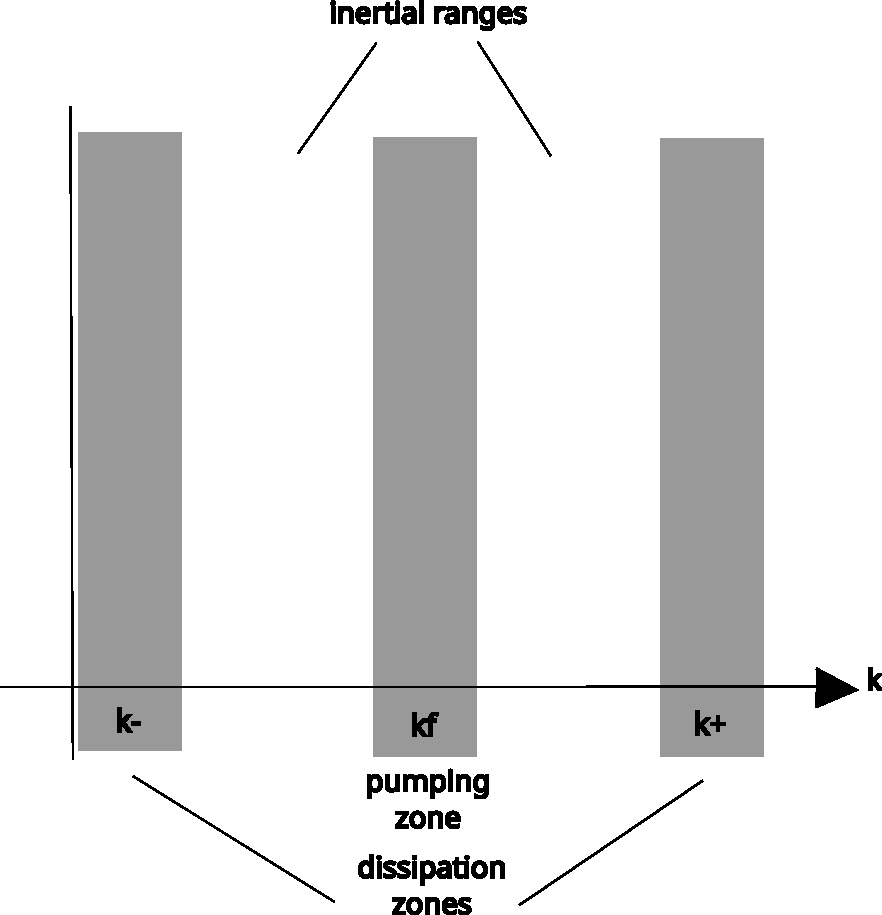
\includegraphics[width=0.5\textwidth]{images/Fjortoft.pdf}
    \caption{Pictorial representation of Fjortoft argument}
\end{figure}

To begin answering the first question we may start with a generic argument due to Fjortoft. We assume the system to be isotropic and concerns ouserlves only with the 
wave vector absolute value\footnote{If until now we meant the whole vector with $k$, now it represents only its modulus.}. We imagine a system with a localized forcing 
around $k_f$ in k-space, inserting per unit time energy density $\Edens_f$ and wave action density $n_f$. Then are present two dissipating regions at $k_-$ and $k_+$
extracting from the system per unit time relatively $\Edens_-$, $\Edens_+$, $n_-$ and $n_+$. We assume $k_- \ll k_f \ll k_+$ so that two inertial ranges are present.\\


Assuming that the dissipating mechanisms are able to fully absorb what is injected in the forcing region, we may require that energy and wave action are conserved:
\begin{align}
    \omga_{k_f}n_f &=  \omga_{k_-}n_- + \omga_{k_+}n_+ \\
    n_f &= n_- + n_+,
\end{align}
where we used $\Edens_k = \omga_k n_k$. A crucial assumption for this argument, true for many physical systems, is that $\omga_k$ is a monotonical function 
of its arguments and it grows as $k$ grows.\\
Let us now pretend that almost all the wave action density is dissipated at $k_+$, i.e. $n_f \simeq n_+$. Using the definition of $\Edens$ 
\begin{equation}
    n_f = \frac{\Edens_f}{\omga_{k_f}} \simeq \frac{\Edens_+}{\omga_{k_+}},
\end{equation}
leading to 
\begin{equation}
    \frac{\Edens_+}{\Edens_f} \simeq \frac{\omga_{k_+}}{\omga_{k_f}}.
\end{equation}
Given that $k_f$ and $k_+$ where assumed to be well separated and monotonicity of $\omga_k$ implies $\omga_{k_+} \gg \omga_{k_f}$, we find 
\begin{equation}
    \Edens_+ \gg \Edens_f,
\end{equation}
implying that more energy is dissipated than what was introduced, clearly paradoxical. This for now only shows that the full wave action flux, if different than zero, cannot 
fully flow from low to high $k$. It does suggests however that the majority of wave action will be transfered towords lower $k$ that where it was introduced, we will 
later prove this in a more rigorous way. \\
Turning to the energy flux let us now pretend that energy density is instead almost fully dissipated at $k_-$, meaning that $\Edens_f \simeq \Edens_-$, we follow the same 
logic as before to find
\begin{equation}
    \Edens_f = \omga_{k_f}n_f \simeq \omga_{k_-}n_- \hspace{2mm} \longrightarrow \hspace{2mm} \frac{n_f}{n_-} \simeq \frac{\omga_{k_-}}{\omga_{k_f}}.
\end{equation}   
Again $\omga_{k_-} \ll \omga_{k_f}$ thus implying the paradoxical conclusion that $n_- \gg n_f$, more wave action is dissipated than introduced. As before this only 
shows that the energy flux cannot fully go towords lower $k$, and it suggests that said flux will mainly move towords high k. We will later prove this as well. \\
This argument hints at the physical picture that we will later draw through more careful mathematical analysis. In a generic system with nonlinear interaction among 
k-modes and monotonical dispersion relation, if some mechanism allow for injection of conserved quantities in a limited region and other mechanisms extract those
same quantities both at much higher and much lower wave number, the nonlinear interaction may allow for out of equilibrium stationary states where energy flow towords high
$k$ and wave action towords low $k$. Even at its early stage we can already appreciate how powerful this result may be, given its generality and the wide array of settings
that can manifest such phenomenology. But let us not get ahead of ouselves, we have for now only a blurred picture of the situation. \\

First we start by the most general way of introducing forcing and dissipation in the kinetic equation. We add a term $\Gamma_k$, resuming within itself the dynamics of 
wave generation and damping, multiplied to $n_k$, as it intuively makes sense that the higher the number of waves of a certain lenght, the more effective the generation
or destruction of them. We thus write
\begin{equation}
    \pt n_k = \coll + \Gamma_k n_k, 
    \label{kineticgamma}
\end{equation} 
where again $\coll$ stands for the collisional integral and the time dependance is implicit. It is easy to convince ourselves that where $\Gamma_k > 0$ it represents the growth rate of waves and 
where $\Gamma_k < 0$ it represents the dampening rate. A torough examinations of the conditions that must be present on $\Gamma_k$ to have a consistent theory
is presentend in \cite{Zakharov}, we here avoid it as to keep this introduction straightforward.\\

Guided by the intuition gathered through Fjortoft's argument, we look for stationary solutions of the kinetic equation with active fluxes of energy or wave action. 
As we expect the fluxes to bring conserved quantities across an eventual inertial range, we study the equation without the $\Gamma_k$ term. Given our choice of locality
on $\Gamma_k$ we make now a reasonable universality assumption, $n_k$ in the inertial range does not depend on the explicit form of the pumping and dissipating term.\\
We look for a solution with a power law spectrum, to this end from now on we assume the system to be isotropic and concern ourselves only with dependance on the wave number 
modulus $k$. Our ansatz is  
\begin{equation}
    n_k = A k^{-\nu}.
    \label{ansatz}
\end{equation}
where $A$ is an arbitrary constant. 
This ansatz was first introduced by Zakharov in 1965 \cite{Zakharov1965}, inspired by similar behavior in hydrodynamics discovered by Kolmogorov on on dimensional grounds 
in 1941 \cite{1991}.\\
A proper analysis would consist in substituting \eqref{ansatz} into \eqref{kinetic} and perform the so-called Zakharov transform, to put the integrand in a form where 
the values of $\nu$ for which $\coll = 0$ are obvious. For an analysis of such method in the general case we remind again the reader to \cite{Zakharov}. \\
\hl{IF THERE IS TIME AT THE END INSERT HERE ZAKHAROV TRANSFORM EXPLANATION}\\
We choose instead the route of dymensional analysis. After inserting our ansatz in the kinetic equation, we perform the change of variables $k_i = q_i k$ to leave a 
dimensionless integral. To proceed we have to restrict the possible forms of the interaction term $\Tint_{k123} = \Tint(k, k_1, k_2, k_3) $, we require it to be an homogeneus 
function of degree $\beta$. Meaning that
\begin{equation}
    \Tint(\lambda k, \lambda k_1,\lambda k_2,\lambda k_3) = \lambda^\beta \Tint(k, k_1, k_2, k_3).
\end{equation}
We assume as well the dispersion relation to be an homogeneus function of degree $\alpha$\footnote{For surface gravity waves $\alpha = \dfrac{1}{2}$ and for the 
nonlinear Schrodinger equation $\alpha = 2$}, this assumption togheter with the isotropy one implies $\omga_k = |k|^{\alpha}$. We obtain 
\begin{multline}
    \coll = 4\pi A^3 k^{3d - 3\nu + 2\beta - d - \alpha} \int \mathrm{S}^3dq_1 dq_2 dq_3 q^{d-1}_1 q ^{d-1}_2 q^{d-1}_3 \\
    |\Tint(1, q_1, q_2, q_3)|^2 q_1^{-\nu}q_2^{-\nu}
    q_3^{-\nu}\left(1 + q_1^\nu - q_2^\nu - q_3^\nu \right) \delta (1 + |q_1|^\alpha - |q_2|^\alpha -|q_3|^\alpha)\delta(1 + q_1 - q_2 -q_3),
\end{multline} 
where we moved to generalized spherical coordinates in $d$ dimensions and $\mathrm{S}$  is the unit radius sphere's surface
resulting from angular integration. 
As for the delta functions, their known property under integration was used:
\begin{equation*}
    \delta(\lambda x) = \frac{1}{\lambda} \delta (x).
\end{equation*}
We will refer in the following to the adimensional integral as $\collad(\nu)$. 
Let us start with the energy flux; with a slight redefinition of the energy density,
to account for spherical coordinates, the continuity equation \eqref{Econtinuity} turns to 
\begin{align}
    &\Edensis_k = \mathrm{S}k^{d-1}k^\alpha n_k \\
    &\pt \Edensis_k + \frac{\partial}{\partial k}  \Pflux_k = 0,
    \label{Econtinuityis}
\end{align}
where $\Pflux_k$ is the radial component in spherical coordinates of the flux vector,
again depending only on the wave vector modulus.\\
By using \eqref{kinetic} we find
\begin{equation}
    \pt \Edensis_k = \mathrm{S} k^{d-1+\alpha} \coll = \mathrm{S} A^3 k^{3d-1-3\nu +2\beta} \collad(\nu),
\end{equation}
that togheter with \eqref{Econtinuityis} and the fundamental theorem of calculus gives 
\begin{equation}
    \Pflux_k = - 4\pi \mathrm{S} A^3 \collad(\nu) \int_{0}^{k} dx x^{3d-1-3\nu +2\beta} = - 4\pi \mathrm{S} A^3 \collad(\nu) 
    \frac{k^{3d+-3\nu +2\beta}}{3d-3\nu +2\beta}.
    \label{KZP}
\end{equation} 
A perfectly analogous process lead to a similar expression for the wave action flux $\Qflux_k$, with a difference in the exponent due to the wave action 
density\footnote{Again slightly modified to account for spherical coordinates} being $\tilde{n}_k=\mathrm{S}k^{d-1}n_k$. The result is
\begin{equation}
    \Qflux_k = - 4\pi \mathrm{S} A^3 \collad(\nu) \frac{k^{3d-3\nu +2\beta-\alpha}}{3d-3\nu +2\beta-\alpha}.
    \label{KZQ}
\end{equation}
We already know that the Rayleigh-Jeans state \eqref{Gibbs} is a stationary solution, hence $\collad(\alpha) = 0$. This implies that in the case of a closed system there are no
fluxes of conserved quantities traversing the system, as to be expected from thermalization. \\ 
Returning to the open system previously discussed we see that nontrivial stationary solutions\footnote{If they exist} must have constant fluxes. If they had null fluxes
there would be no transfer of energy and wave action across the inertial range, incompatible with the presence of a forcing region and a dissipating one. If instead the fluxes
were to be dependant on $k$ in the inertial range, there would be no balance between the quantities flowing into a certain mode $k$ and those leaving it, leading to 
$\pt n_k \neq 0$. \\
Looking at \eqref{KZP} and \eqref{KZQ} we see that the only way a possible stationary solution could yeald finite flux is to have an exponent $\nu$ which is a zero of 
the denominator, we thus obtain the 2 scalings
\begin{align}
    \nu_P &= \frac{2}{3}\beta + d, \\
    \nu_Q &= \frac{2}{3}\beta + d - \frac{1}{3}\alpha.
\end{align}
Setting a general constant value for the fluxes, applying l'Hopital rule and assuming that what we found are really the exponent of stationary solutions, i.e 
$\collad(\nu_P)=\collad(\nu_Q)=0$, we find 
\begin{align}
& \lim_{\nu \leftarrow \nu_P}  \Pflux_k = \Pflux_0 = \frac{4}{3}\pi \mathrm{S} A^3 \collad'(\nu_P), \label{limP}    \\
& \lim_{\nu \leftarrow \nu_Q}  \Qflux_k = \Qflux_0 = \frac{4}{3}\pi \mathrm{S} A^3 \collad'(\nu_Q), \label{limQ}
\end{align}
showing that we should also check in the specific cases that the first derivative of the dimensionless collision integral with respect to the power law solution's 
exponent must be finite. The value of said derivative determines the direction of the flow of the relative conserved quantity. \\
Expressing the generic prefactor $A$ as a function of the flux in each case and renaming it properly we finally obtain the famous Kolmogorv-Zakharov solutions 
\begin{align}
    &n_k^P = C_{KZ}^P \Pflux_0^{\frac{1}{3}} k^{\frac{2}{3}\beta + d}, \label{KZPsol}\\
    &n_k^Q = C_{KZ}^Q \Qflux_0^{\frac{1}{3}} k^{\frac{2}{3}\beta + d - \frac{1}{3}\alpha}. \label{KZQsol}
\end{align}
Where $C_{KZ}^P = \left(\frac{3}{4\pi\collad'(\nu_P)}\right)$ and 
$C_{KZ}^Q = \left(\frac{3}{4\pi\collad'(\nu_Q)}\right)$ are the Kolmogorov-Zakharov constants. Those state are often called cascade solutions, as they correspond to conserved quantities flowing
(or cascading) across k-space.\\
The value of $\Pflux_0$ and $\Qflux_0$ will instead depend on the specific mechanisms at work in the pumping an damping regions. Their value may be extimated 
from the specific form of $\Gamma_k$. \\
For example for the energy flux one has to look at the continuity equation outside of the inertial range, easily obtainable from \eqref{kineticgamma} 
\begin{equation}
    \pt \Edensis_k + \frac{\partial}{\partial k}  \Pflux_k = \Gamma_k \Edensis_k. 
    \label{continuitygamma}
\end{equation}
When in a stationary solutions the time derivative part is null and by finite integration from a generic $k_0$ to infinity we obtain
\begin{equation}
\Pflux_{\infty} - \Pflux_{k_0} = \int_{k_0}^{\infty} dk \Gamma_k \Edensis_k.
\end{equation}
By placing $k_0$ in the inertial range it follows $\Pflux_{k_0} = P_0$ and recognizing that in any reasonable physical setting $P_{\infty} = 0$ we find
\begin{equation}
    \Pflux_0 = - \int_{k_0}^{\infty} dk \Gamma_k \Edensis_k = \int_{0}^{k_0} dk \Gamma_k \Edensis_k,
\end{equation}
where we also added the result obtained by integrating from zero to $k_0$, the two expression are not at odd with each other, as if we require conservation of energy 
and integrate from zero\footnote{As we are still working in the isotropic case} to infinity the equation \eqref{continuitygamma}, we obtain the condition 
\begin{equation}
    \int_{0}^{\infty} dk \Gamma_k\Edensis_k = 0, 
\end{equation}
showing that the two integrals for $\Pflux_0$ coincide. \\
The whole discussion applies equally to $\Qflux_0$ and its continuity equation, resulting in 
\begin{equation}
    \Qflux_0 = - \int_{k_0}^{\infty} dk \Gamma_k \tilde{n}_k = \int_{0}^{k_0} dk \Gamma_k \tilde{n}_k,
\end{equation}
where the two integrals coincide provided that 
\begin{equation}
    \int_{0}^{\infty} dk \Gamma_k\tilde{n}_k = 0
\end{equation}
is satisfied. \\

Let us be clear. As already said we did not prove that \eqref{KZPsol} and \eqref{KZPsol} are solutions to the kinetic equation, we have only shown that if 
an inertial interval exist among regions in which energy and wave action are injected and extracted, the only consisten form a solution could take in such 
interval to have a constant flux of conserved quantities is either \eqref{KZPsol} or \eqref{KZPsol}. \\
Looking at the formulas \eqref{limP} and \eqref{limQ} we see that in any region where one of the fluxes is constant, the other must be null. This information, coupled 
with the previously presented Fjortoft's argument, fixes the direction for cascade solutions of theories with $\omga_k$ monotonical. From the expression of the fluxes 
we know that each quantity must flow almost completely upward or downward k-space, but Fjortoft's argument prohibits one direction for  each of them. Thus energy
will be flowing towords high k, whereas wave action will flow towords low k. As historically the first cascade solutions to be discovered where of the first kind, 
in this context energy cascade is called a direct cascade, conversely the wave action one is called an inverse cascade. \\

Even after possibly proving that what we found actually are solutions, it must be checked case by case that the collisional integral is converging in the first place, 
in other words the theory must be local, in the sense that points far removed from each other in k-space must have vanishing influence on each other. \\
When checking if this is the case with the general system we have been studying, some bounds are posed on the parameters $\alpha$ and $\beta$ that we introduced.
Those bounds identify what is called a locality window and every healthy theory's parameters should fall in such window. We mention this because 
the presence of this interval is not granted when analyzing higher perturbative orders.\\ 
Many topics were not discussed, among them the stability problem of the KZ solutions and the analysis of anisotropic systems. The reader is directed to the 
already cited references for an in depth discussion of those and many more topics.

Weak turbulence theory has been successfull in explaining experimental findings in a number of settings. Some examples are Rossby waves in a rotating fluid, internal waves 
in a stratified fluid, capillary waves, gravity surface waves in the ocean and quantum bose gases. \\
\hl{CITATIONS TO BE ADDED, MAYBE IT WOULD MAKE SENSE TO CITE ONLY 4 WAVE SYSTEMS, ASKS PROFESSOR FOR EXAMPLES AND HOW 
TO USE PLOTS FROM PAPERS, MAYBE THERE SHOULD BE ADDED SOME REMARKS ON THE LIMITS OF WWT (SOLITONS, STRONG TURBULENCE)}


%chapter2
% !TEX root = ../../thesis.tex

\newpage
\vphantom{}
\section{Beyond the leading order}
Deriving the wave kinetic equation by truncating perturbation theory at higher orders is not an easy feat. Calculations become quickly extremely cumbersome. Approaches 
based on classical diagrammatic methods were developed in \cite{Zakharov1975} and \cite{Gurarie:1994ut}. Lately techniques exploiting Feynman diagrams were developed in
\cite{Rosenhaus2023}, \cite{Rosenhaus:2022uwa} and \cite{Rosenhaus:2023sik}. This new methods allow for a relatively fast derivation of higher order kinetic equations.
Such equations and their validity are discussed in \cite{Rosenhaus:2023pdj}. The possibility of gaining insight into the strong turbulent regime by resumming 
part of the corrections was investigated instead in \cite{Rosenhaus:2025mgj}. \\
The focus of this chapter is to introduce the computational tools to consistently derive kinetic equations with contributions from higher powers of the coupling. 
The methods of \cite{Rosenhaus2023} are discussed in a generic four wave system. First we show \hl{MAYBE CITE SIGGIA ROSEN MARTIN} how to map the derivation of the kinetic equation into
the task of evaluating correlators in a Quantum Field Theory model. The basic idea is that a nonlinear system coupled to a random forcing may be regarded as 
a statistical theory were the normal variables of the orginal system inherit the stochastic properties of the forcing. If the system spectrum in Fourier space is continous
a path integral approach may be implemented, allowing for the usage of the well developed machinery of QFT perturbation theory.\\
After introducing and commenting the Feynman rules of the model, we calculate two and four points 
correlation functions up to the first nontrivial higher order to derive the corresponding kinetic equation. The resulting theory can be said to account 
not only for direct four wave interactions,as \eqref{kinetic}, but also for the exchange of virtual waves among different modes. We end the chapter by briefly discussing the implications
of this corrected equations for the KZ spectra. \\  
\subsection{Path integral formulation of weak turbulence theory}

There are many ways to derive the kinetic equation for weakly interactive waves. One of them is by looking at the late time behaviour of the same nonlinear system
coupled to a complex gaussian forcing and some dissipation, as in \cite{Zakharov1975} we write the modified e.o.m.s (already in the continuum limit)
\begin{equation}
    \pt a_k + i \omga_k a_k = -i \sum_{123}\Tint_{k123} \aonestar\atwo\athree \delta^{k1}_{23} + f_k(t) - \gamma_k a_k
    \label{eoms}
\end{equation}

and impose guassian statistics on the forcing
\begin{equation}
    \langle f_k(t)f_p(t')\rangle = \F_k \delta(k-p)\delta(t-t').
\end{equation}
solving the system perturbatively and looking at a big enough $t$, equation \eqref{kinetic} is recovered. \\
The forcing and dissipation introduced this way are not of physical importance and have nothing to do with the $\Gamma_k$ term responsible 
for the energy and wave action cascades. The contribution of $f_k$ is to introduce randomness into the system, in place of the explicit RPA assumption. 
The last step of the derivation then removes this nonphysical elements by taking the limit of both $\F_k$ and $\gamma_k$ to zero, while keeping their ratio finite as
to obtain a finite wave density $n_k$. \\  
\hl{SCRIVI CONTO SE C'E' TEMPO} \\
This is the starting point adopted by Rosenhaus and Smolkin in \cite{Rosenhaus2023} to access, with manageable calculation, higher orders in perturbation theory. We will 
follow their method in this section.\\
The basic idea is to reformulate the theory in the language of path integrals, to then move the statistics from the forcing to the canonical variables $\ak$. We start by
explicitly writing the probability distribution for a given $f_k(t)$ functional form as 
\begin{equation}  
    \mathrm{P}[f] \sim e^{-\int dt \sum_k \frac{|f_k(t)|^2}{\F_k}},
\end{equation}
Where instead of an integration on $k$, even if we are in the continuum limit, we write a sum. This choice is to improve clarity in the cumbersome formulas 
we will later write, but sums should always be intended as integrals. We write the expectation value of a general composition of variables $O(a)$ \footnote{
    In general it could be the composition of various $\ak = ak(t)$ at different wave numbers and different times.
} as 
\begin{equation}
    \langle O(a) \rangle = \frac{1}{\mathrm{Z}}\int \D f \D f^* \mathrm{P}[f] O(a), 
\end{equation}
where the integration measure $\D f$ is a formal sum over all possible functions $f_k(t) = f(k,t)$ and $\mathrm{Z}$ is a normalization constant. If $k$ and $t$ instead of continous variables were discrete labels $i$ and $j$,
the integration measure would be the product $\prod_{ij}d f_{ij}$, running over all the possible values of the labels. \\
We want the $a$ variables to satisfy the equations of motion, we may impose so by first defining a function $\Ef$ as
\begin{equation}
    \Ef = \pt a_k + i \omga_k a_k +i \sum_{123}\Tint_{k123} \aonestar\atwo\athree \delta^{k1}_{23} - f_k(t) + \gamma_k a_k,
    \label{Eeffe}
\end{equation}  
so that the requirement that $\ak$ is a solution of the e.o.m.s may be expressed through a functional $\delta$ imposing $\Ef = 0$. We also need to add an integration measure
$\D \Ef \D \Efstar$ to guarantee the normalization of the probability distribution. The result for a generical expectation value is
\begin{equation}
    \langle O(a) \rangle = \frac{1}{\mathrm{Z}}\int \D f \D f^* \D \Ef \D \Efstar \mathrm{P}[f] O(a)\delta(\Ef)\delta(\Efstar).
\end{equation} 
It is important to notice that we are explicitely writing a measure for a variable and another for its complex conjugate. It is customary that each functional integration
represents an infinity of ordinary integrations of the same cardinality of a line. Thus complex variables require a double measure each\footnote{We formally use a variable 
and its conjugate instead of its real and imaginary part in the same way as one can formally describe the complex plane by using $z$ and $z^*$ instead of x and y.}.\\
\begin{comment}
To ease the upcoming computation we perform the change of variables 
\begin{equation}
    \left(\Ef,\Efstar\right)\rightarrow \left( \text{Re}\{Ef\},\text{Im}\{\Ef\} \right),
\end{equation}
that obviously has a unitary Jacobian\footnote{It consists in an infinite set of transformations $(z, z^*)\rightarrow (x,y)$.}
\end{comment}
Given that we desire a theory where the dynamical variables are the $a$s, we perform a change of coordinates from $\left(\Ef,\Efstar \right)$
to $\left( \anorm, \astar\right)$, resulting in 
\begin{equation}
    \langle O(a) \rangle = \frac{1}{\mathrm{Z}}\int \D f \D f^* \D \anorm \D\astar  \mathrm{P}[f] O(a)\delta(\Ef)\delta(\Efstar)
    \left| \frac{\partial \left( \Ef,\Efstar\right)}{\partial \left( \anorm, \astar\right)}\right|.
    \label{expect1}
\end{equation}
The Jacobian has to interpreted as the matrix 
\begin{equation}
     \frac{\partial \left( \Ef,\Efstar\right)}{\partial \left( \anorm, \astar\right)} = 
    \renewcommand{\arraystretch}{1.8}  % Aumenta la distanza verticale
    \setlength{\arraycolsep}{6pt}     % Aumenta la distanza orizzontale
    \begin{pmatrix}
        \frac{\partial \Ef}{\partial \anorm}  & \frac{\partial \Efstar}{\partial \anorm} \\
        \frac{\partial \Ef}{\partial \astar}  & \frac{\partial \Efstar}{\partial \astar}
    \end{pmatrix}
,
\label{Jacobian}
\end{equation}
where each component is in turn a matrix with infinitely many rows and columns\footnote{We are again interpreting a function as a vector with infinite elements.}. \\
Thanks to Sylvester's formula we know that 
\begin{equation}
    \renewcommand{\arraystretch}{1.8}  % Aumenta la distanza verticale
    \setlength{\arraycolsep}{6pt}     % Aumenta la distanza orizzontale
    \left|
    \begin{pmatrix}
        \frac{\partial \Ef}{\partial \anorm}  & \frac{\partial \Efstar}{\partial \anorm} \\
        \frac{\partial \Ef}{\partial \astar}  & \frac{\partial \Efstar}{\partial \astar}
    \end{pmatrix}
    \right|
    = \left| \frac{\partial \Ef}{\partial \anorm} \frac{\partial \Efstar}{\partial \astar} - \frac{\partial \Efstar}{\partial \anorm} 
    \frac{\partial \Ef}{\partial \astar}\right|.
    \label{sylvester}
\end{equation}
To calculate the determinant of the Jacobian we thus have to evaluate the single elements of \eqref{Jacobian}. To do so we first discretize time in \eqref{Eeffe}, obtaining
\begin{equation}
    \Ef (t) \longrightarrow \Delta t \mathrm{E}_f^{i} = a_k^i - a_k^{i-1} + 
    \Delta t\left(i \frac{\delta \Ham}{\delta a_k^{i-1}} - f_k^{i-1} + \gamma_k^{i-1}a_k^{i-1}\right).
    \label{discretization}
\end{equation}
As $\mathrm{E}_i$ does not depend on any $a_k^{j}$ with $j > i$ both the diagonal terms in \eqref{Jacobian} are triangular matrices, moreover the diagonal only contains 
ones as the dependance on $a_k^{i}$ is linear. \\
The remaining elements of the \eqref{Jacobian} are triangular matrices with the diagonal containing only zeroes, as
$\mathrm{E}_f^{i*}$ and  $\mathrm{E}_f^{i}$ do not depend on $a_k^{i}$  and $a_k^{i*}$ respectively. Knowing that the product of such two matrices is null lets us remove it 
from \eqref{sylvester}. \\
Given that the determinant of a triangular matrix is equal to the product of its diagonal elements we find 
\begin{equation}
    \renewcommand{\arraystretch}{1.8}  % Aumenta la distanza verticale
    \setlength{\arraycolsep}{6pt}     % Aumenta la distanza orizzontale
    \left|
    \begin{pmatrix}
        \frac{\partial \Ef}{\partial \anorm}  & \frac{\partial \Efstar}{\partial \anorm} \\
        \frac{\partial \Ef}{\partial \astar}  & \frac{\partial \Efstar}{\partial \astar}
    \end{pmatrix}
    \right|
    = \left| \frac{\partial \Ef}{\partial \anorm} \frac{\partial \Efstar}{\partial \astar}\right|
    = \left| \frac{\partial \Ef}{\partial \anorm} \right| \left|\frac{\partial \Efstar}{\partial \astar}\right|
    = 1,
\end{equation} 
thus letting us remove the Jacobian from \eqref{expect1}.\\
We now use the functional integral representation of $\delta$
\begin{equation}
    \delta(\Ef)\delta(\Efstar) = \int \D \eta\D \eta^* e^{i\int dt \sum_{k}\left( \eta_k^{}\Efstar +\eta_k^* \Ef\right)}
\end{equation}
to obtain 
\begin{equation}
    \langle O(a) \rangle = \frac{1}{\mathrm{Z}}\int \D f \D f^* \D \anorm \D\astar\D \eta\D \eta^*  O(a)
    e^{-\int dt \sum_k \left( \frac{|f_k(t)|^2}{\F_k} - i\eta_k^{}\Efstar -i\eta_k^* \Ef \right)}.
    \label{expect2}
\end{equation}
$\Ef$ only depends on $f_k$ linearly by construction. To integrate out the forcing from the theory we notice that the exponent's part depending on $f_k$
can be reformulated partly as a Gaussian. 
Let us look at the same problem in a simplified setting where $(f_k^{},f_k^*)  \rightarrow (z, z^*)$, $(\eta_k^{}, \eta_k^*) \rightarrow (u, u^*)$ and $\F_k \rightarrow c$.
The part of the exponent under consideration is then
\begin{equation}
    -\frac{zz^*}{c} + iuz^* + iu^*z = -\frac{1}{c} \left(z - iuc \phantom{z^*}\hspace{-3mm}\right)\left(z^* - iu*c \right) - uu^*c,
\end{equation}
where we completed the square. The procedure is easily extendable to the infinite dimensional case. After integrating out the Gaussian integral and absorbing it into the 
normalization constant\footnote{With the difference that there is not a closed form expression 
for the value of the integral, we only now that under a change of coordinates there is a noninteracting free theory. Given that this theory is decoupled 
from the dynamical variables we are interested in,
we can just ignore it. This is what we mean by absorbing it into the normalization constant.}  we find
\begin{equation}
    \langle O(a) \rangle = \frac{1}{\mathrm{Z}}\int\D \anorm \D\astar\D \eta\D \eta^*  O(a)
    e^{-\int dt \sum_k \left( \eta_k^{}\eta_k^* F_k - i\eta_k^{}\Efstarz -i\eta_k^* \Efz \right)},
    \label{expect3}
\end{equation}
where $\Efz$ corresponds to $\Ef$ without forcing term. In an analogous way, by again completing the square, the integral over $\eta$ and $\eta^*$ may be performed and 
absorbed into the normalization constant.
The result is 
\begin{equation}
    \langle O(a) \rangle = \frac{1}{\mathrm{Z}}\int\D \anorm \D\astar O(a)
    e^{-\int dt \Lag},
    \label{expect}
\end{equation} 
with $\Lag$ defined as 
\begin{equation}
    \Lag = \sum_k \frac{|\Efz|^2}{\F_k}.
    \label{Lag}
\end{equation}
What we have found is a statistical theory of the dynamical variables $\anorm$ and $\astar$ in the continuum limit. Through a Wick rotation $t \rightarrow \tau = it$ we 
may turn it into a Quantum Field Theory, where the machinery of Feynman diagrams can be utilized to perform efficient perturbative calculations.\\

\subsection{Feynman rules} 

Our objective is still the kinetic equation. Starting from the original equations of motions \eqref{eoms}, without forcing and dissipation
\begin{equation}
    \pt a_k + i \omga_k a_k = -i \sum_{123}\Tint_{k123} \aonestar\atwo\athree \delta^{k1}_{23},
\end{equation}
multiplying it for $\akstar$ and summing its complex conjugate we obtain
\begin{equation}
    \pt \ak \akstar = -2 \text{Im}\left( \sum_{123}\Tint_{k123}\ak \aone \atwostar \athreestar \delta^{k1}_{34} \right).
\end{equation} 
By averaging over all possible realizations and expliciting the time dependences we find
\begin{equation}
    \pt \langle \ak(t) \akstar(t) \rangle = -2 \text{Im}\left( \sum_{123}\Tint_{k123}\langle\ak(t) \aone (t)\atwostar(t) \athreestar (t)\rangle\delta^{k1}_{34} \right),
    \label{kineticprototype}
\end{equation}
where on the l.h.s. we can see the definition of $n_k(t)$ given in \eqref{wavdef}. We notice from this equation how any order of the kinetic equation can be obtained 
by evaluating four points functions at equal times, togheter with the RPA assumption. Those four points function can be evaluated by the path integral statistical theory 
derived in the last section, where the RPA assumption is recovered through the gaussian statistics over the forcing. Of course we will have to properly 
switch off the contributions form the forcing variance $\F_k$ and the dissipation $\gamma_k$ to obtain results consistent with the first chapter. \\
The good news is that through Feynman diagrams we can calculate four point functions with relative ease. In this section we will write and explain the Feynman rules. 
A full derivation would imply an introduction to Quantum Field Theory, a task out of the scope of this thesis. The reader not familiar with the topic is directed to 
the variety of existing books (for example \cite{Bjorken:1965zz}). \\

We start by expliciting writing $\Lag$ as
\begin{equation}
    \Lag = \sum_k \frac{|\Efz|^2}{\F_k} = \sum_k \frac{1}{\F_k} \left| \pt a_k + i \omga_k a_k + i \sum_{123}\Tint_{k123} \aonestar\atwo\athree \delta^{k1}_{23} \right|^2.
\end{equation} 
Regrouping the different terms order by order $\Lag$ becomes 
\begin{equation}
    \Lag = \Lag_0 + \Lag_1 + \Lag_2.
\end{equation}
with, by extensive usage of the symmetries of $\Tint$ and dummy variables, 
\begin{align}
    \Lag_0 &= \sum_k\frac{1}{\F_k} \left| \Dcov_k a_k  \right|^2, \\
    \Lag_1 &= \frac{i}{2}\sum_{k123}\Tint_{k123}\left( \frac{\Dcovd_k}{\F_k} + \frac{\Dcovd_1}{\F_1} - \frac{\Dcov_2}{\F_2} - \frac{\Dcov_3}{\F_3} \right)
    \akstar \aonestar \atwo \athree, \\
    \Lag_2 &= \sum_{k123456} \frac{1}{\F_k}\Tint_{123k}\Tint_{k456}\aonestar \atwostar \athree \afourstar \afive \asix. 
\end{align}
In this last set of equations we defined 
\begin{equation}
    \Dcov_k a_k = \left(\pt + i\omga_k+ \gamma_k\right)\ak
\end{equation} 
and $\Dcovd_k \akstar$ is its complex conjugate. Moreover in every expression 
like $\frac{\Dcovd_1}{\F_1}\akstar \aonestar \atwo \athree$ the $\Dcovd_k$ always acts only on the normal variable bearing its own argument. \\

We shall directly write the Feynman rules in frequency space, as the calculations are easier this way. We will need to transform back to $t$-space every 
correlator we obtain.\\
Up until now we have been using $\omga_k$ and $\omga_i$ as $\omga(k)$ and $\omga(k_i)$, to avoid introducing unnecessary confusion the 
fourier transform frequency will be named $\omgatt$ . Therefore the fourier transform of a function of $t$ will be a function of $\omgatt$ and the fourier 
transform of a function of $t_i$ will be a function of $\omgatt_i$. \\
The propagator of the free theory may be obtained inverting the quadratic part of the Lagrangian ($\Lag_0$), yealding 
\begin{equation}
    G_{k1}(t_1 - t_2) = \langle \akstar(t_1)\aone(t_2)\rangle = \F_k \delta(k-k_1)\int \frac{d \omgatt}{2\pi}\frac{e^{i\omgatt(t_1 - t_2)}}
    {\left(\omgatt -\omga_k + i\gamma_k \right)\left(\omgatt -\omga_k-i \gamma_k\right)}. 
    \label{propspace}
\end{equation}
It is instructive to look at its explicit form. We use Jordan's lemma to close the integration path in the upward or downward half of the complex plane, obtained by 
making the variable $\omgatt$ complex, depending on the sign of $t_1 - t_2$. We then use the residue theorem to give an explicit form to the propagator, obtaining
\begin{multline}
    G_{k1}(t_1 - t_2) = \langle \akstar(t_1)\aone(t_2)\rangle = \\
    \frac{\F_k}{2\gamma_k}\delta(k-k_1)\left(\theta(t_1-t_2)e^{i(\omga_k + i\gamma_k)(t_1 - t_2)}
    +\theta(t_2-t_1)e^{i(\omga_k - i\gamma_k)(t_1 - t_2)}\right),
\end{multline}  
where $\theta(x-y)$ is the Heavyside's function. Given the definition of the wave action density as an equal time two point correlator, we may conclude that for a 
free theory
\begin{equation}
    n_k = \frac{F_k}{2\gamma_k}.
    \label{freenwav}
\end{equation}
This makes perfectly sense, as in the absence of nonlinear terms there is no exchange of energy among modes, and thus the wave action density at a given $k$ is determined
only by the ratio of the forcing variance (how many waves are introduced at $k$) and the dissipation (how many waves are destroyed at $k$). \\
The Fourier transform of the free theory propagator is
\begin{equation}
    \tilde{G}^0_{k1}(\omga)=\delta(k-k_1)\D^0_k=\delta(k-k_1)\F_k|\G_k|^2,
    \label{prop}
\end{equation}  
where we defined 
\begin{equation}
    \G_j = \frac{i}{\omgatt + i\gamma_j -\omga_j}.
\end{equation}
The full Feynman rules in frequency space are\\
\begin{center}
    \begin{tikzpicture}
    \begin{feynman}
      \vertex[label=left:{\(1\)}] (i) at (-0.75,0);
      \vertex [right=1.5cm of i] (f);
  
      \diagram* {
        (i) -- [fermion, arrow size=1.1pt] (f);
      };
    \end{feynman}
  
     % Arrow pointing to the first equation
    \draw[->] (2,0) -- (3,0);
    % First equation on the right
    \node at (6,0) {\(F_1|\G_1|^2\)};
    \begin{feynman}
      \vertex (v1) at (0,\ytwo);
      \vertex [below left=1cm of v1] (ii4){\(4\)};
      \vertex [below right=1cm of v1] (ii3) {\(3\)};
      \vertex [above left=1cm of v1] (ff1) {\(1\)};
      \vertex [above right=1cm of v1] (ff2) {\(2\)};

      \diagram* {
        (ii4) -- [fermion, arrow size=1.1pt] (v1) -- [fermion, arrow size=1.1pt] (ff1),
        (ii3) -- [fermion, arrow size=1.1pt] (v1) -- [fermion, arrow size=1.1pt] (ff2),
      };
    \end{feynman}

    \draw[->] (2,\ytwo) -- (3,\ytwo);

    \node at (8,\ytwo) {\begin{math}\text{-}i\pi\Tint_{1234}\left(\dfrac{1}{\G_1^*\F_1^{}}+\dfrac{1}{\G_2^*\F_2^{}}-\dfrac{1}{\G_3^{}\F_3^{}}
        -\dfrac{1}{\G_4^{}\F_4^{}}\right)\delta(\delomegatt^{12}_{34})\delta^{12}_{34}\end{math}};
  
    \begin{feynman}
    % Central vertex
      \vertex (center) at (0,\y);

      % Define six external vertices at 60-degree intervals around the center
      \vertex[label=\(2\)] (i2) at ($(center) + (90:1)$);   % 90 degrees (top)
      \vertex[label=left:\(1\)] (i1) at ($(center) + (150:1)$);  % 150 degrees (top-left)
      \vertex[label=left:\(6\)] (f6) at ($(center) + (210:1)$);  % 210 degrees (bottom-left)
      \vertex[label=below:\(5\)] (f5) at ($(center) + (270:1)$);  % 270 degrees (bottom)
      \vertex[label=right:\(4\)] (i4) at ($(center) + (330:1)$);  % 330 degrees (bottom-right)
      \vertex[label=right:\(3\)] (f3) at ($(center) + (30:1)$);   % 30 degrees (top-right)

    % Draw the interactions (lines) between the central vertex and the six external vertices
      \diagram*{
        (i4) -- [fermion, arrow size=1.1pt] (center) -- [fermion, arrow size=1.1pt] (f3),
        (i1) -- [fermion, arrow size=1.1pt] (center) -- [fermion, arrow size=1.1pt] (f6),
        (i2) -- [fermion, arrow size=1.1pt] (center) -- [fermion, arrow size=1.1pt] (f5),
      };
    \end{feynman}

    \draw[->] (2,\y) -- (3,\y);

    \node at (6,\y) {\(\text{-}\sum_{k}\limits\dfrac{\Tint_{123k}\Tint_{k456}}{F_k}2\pi\delta(\delomegatt^{124}_{356})\delta^{12}_{3k}\delta^{k4}_{56}\)};
  
  \end{tikzpicture} 
\end{center}
where $ \delomegatt^{124}_{356} = \omgatt_1 + \omgatt_2 + \omgatt_4 - \omgatt_3 - \omgatt_5 - \omgatt_6$. \\

In the QFT interpretation the deltas over $\omgatt$ and $k_i$ enforce conservation of energy and momentum in any given process. To calculate an $n$-points 
correlation function one has to draw all topologically inequivalent connected diagrams with $n$ external legs, i.e all diagrams that cannot be continously deformed into each other.
Those diagrams may be assembled only through the vertices present in the Feynman rules. To every line composing a diagram a number $i$ is associated,
meaning that every mathematical expression represented by that line is a function of $k_i$ and $\omgatt_i$. Every vertex corresponds to the mathematical expressions 
written above, every external or internal line corresponds to the insertion of a propagator in fourier space $(k, \omgatt)$. For every internal line bearing a number 
$i$, an additional integration $\sum_i \int \frac{d\omgatt_i}{2\pi}$ is to be performed. Additionaly a numerical factor has to be introduced accounting for all the possible 
ways of attaching the external legs to the vertices and external lines obtaining equivalent diagrams. \\
The perturbative order of a given diagram\footnote{Thus also of the mathematical expression it represents.} is equal to $q + 2s$ , where $q$ is the number of quartic vertices 
and $s$ is the number of sextic ones. In the first case only a coupling $\Tint$ appears in the rules and in the second case two of them are present. 
We will now turn to the calculation and analysis of the two and four points functions, in order to obtain a kinetic equation. \\

\subsection{Two points functions}
Let us start by calculating the first order correction to the two points function, the only diagram to consider is the one in figure \ref{fig:oneloop2}. It is made 
of three lines, one of which is internal, and a quartic vertex where $k_3 = k_2$ and $k_1 = k_4$. Given that the number of holes in a diagram grows with the perturbative order, this is usually called a one loop diagram
\footnote{Another common name is NLO contribution, short for next to leading order.}.\\
\begin{figure}[ht]
    \centering
    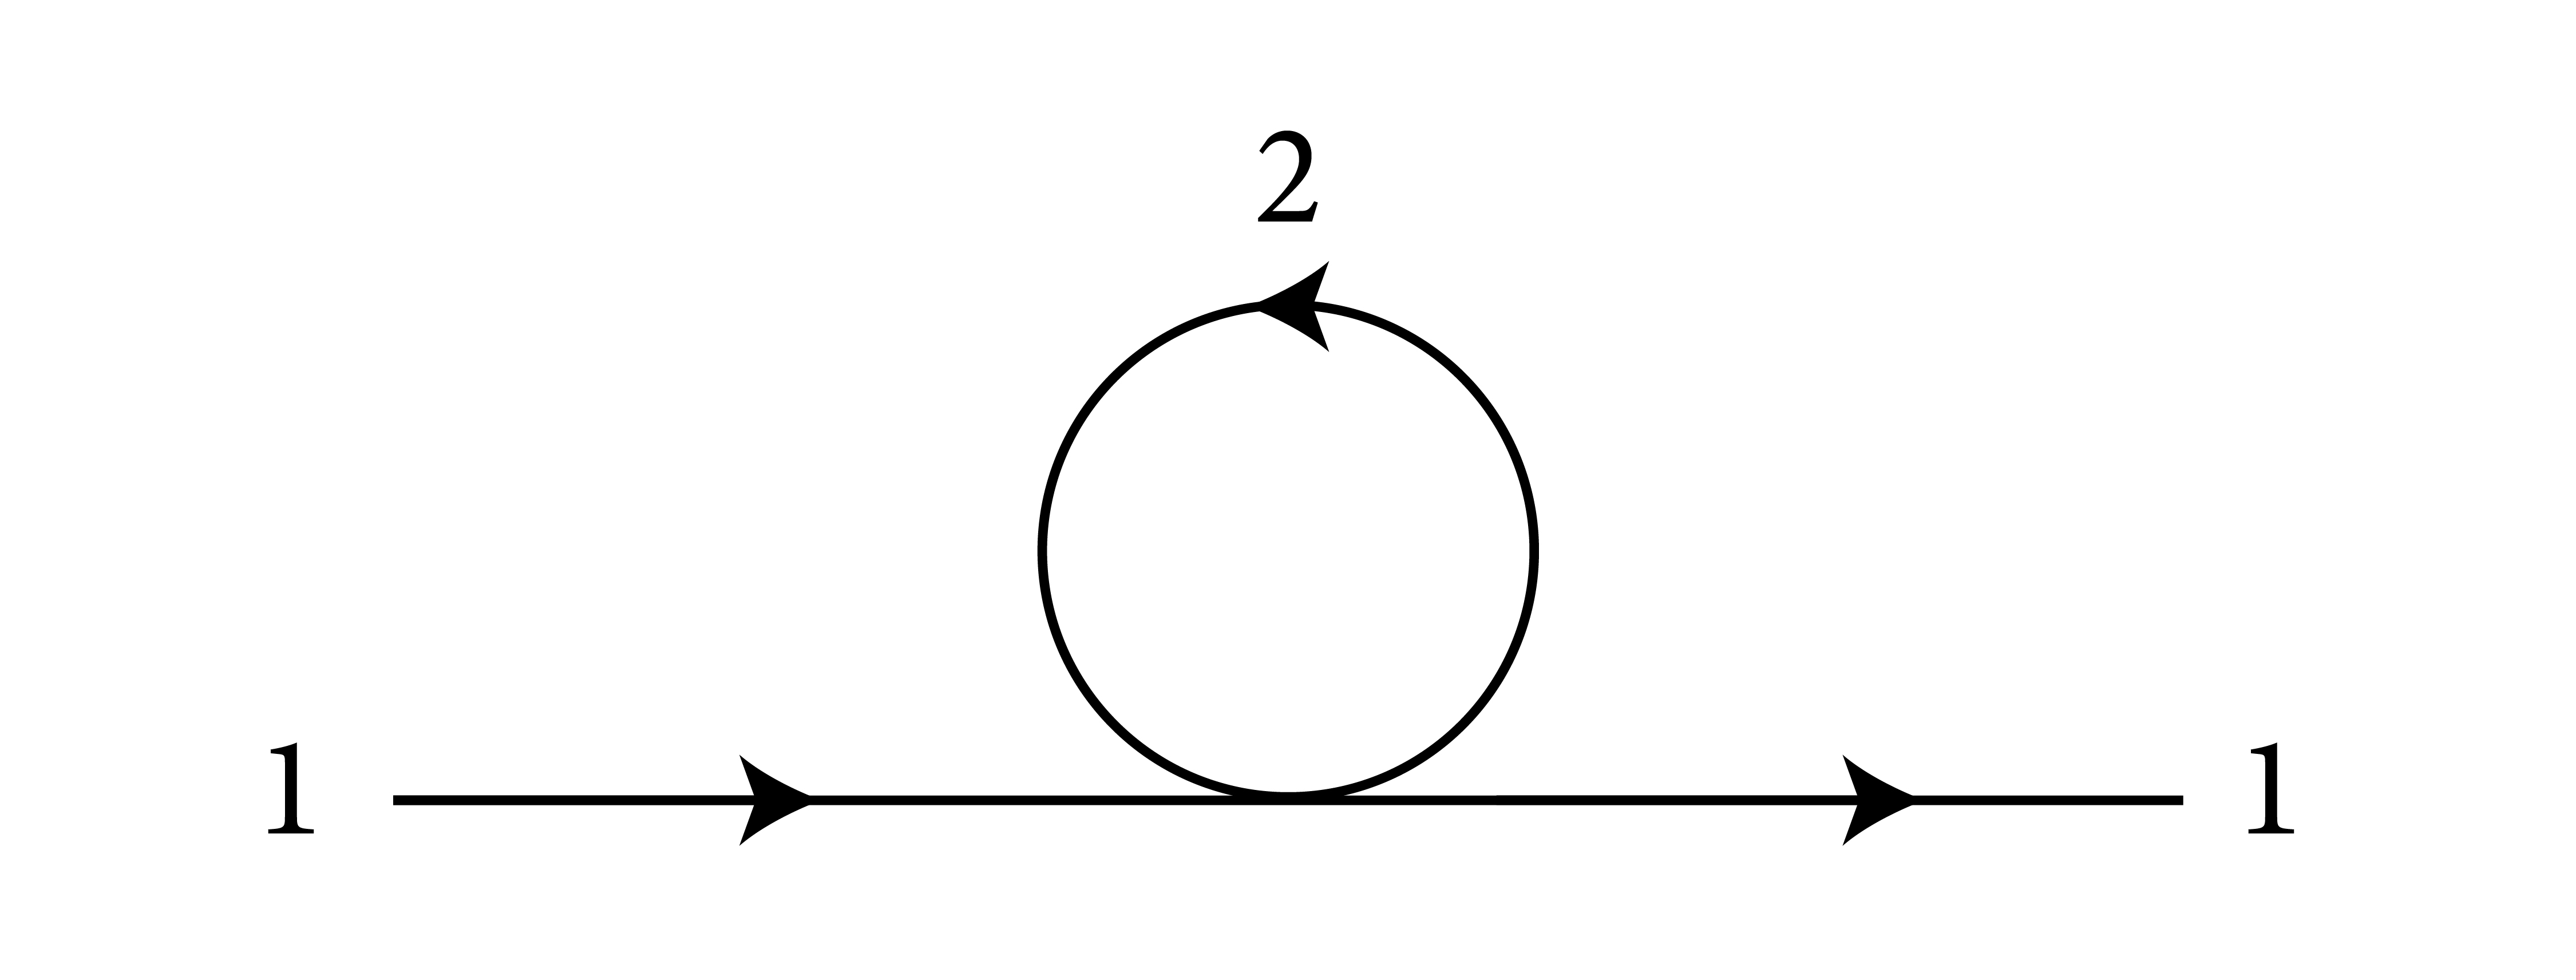
\includegraphics[width=0.6\textwidth]{images/2pointsoneloop.jpg}
    \caption{One loop correction to the two points function.}
    \label{fig:oneloop2}
\end{figure}
We are considering two correlators evaluated at the same points in $k$-space, since our objective is the term present in the r.h.s. of \eqref{kineticprototype}. 
In this case there always will be a delta arising from the diagrams whose argument is zero. This delta is the result of momentum conservation.
For this reason we will be dealing with a $\D_k$ defined as in \eqref{prop} instead of the full propagator\footnote{In equation \eqref{prop} we defined it 
with a zero superscript to indicate it was for the free theory, for the full propagator the definition would be $\tilde{G}_{k1}(\omga)=\delta(k-k_1)\D_k$},
ignoring the infinity arising from the aforementioned delta. \\
Using the Feynman rules explained in the last section, the form of the one loop correction to the two points function is
\begin{equation}
    \D_1^{1} = -4\frac{i}{2} \D^0_1\D^0_1 \sum_{2} \int \frac{d\omgatt_2}{2\pi} \Tint_{1221}\D^0_2\left[\frac{1}{\F_1}\left( \frac{1}{\G_1^*} - \frac{1}{\G_1}\right) +
    \frac{1}{\F_2}\left( \frac{1}{\G_2^*} - \frac{1}{\G_2}\right) 
    \right],
\end{equation}
\hl{THERE IS STILL A MISSING 2PI}\\
where the factor of four is the result of two possible ways of choosing the "incoming" particle and two possible ways of choosing the "outgoing" one.
%where the factor of two in front of the expression is the result of a factor of four, introduced to account for all possible ways to attach the external lines to the vertex 
%and obtain the same diagram, devided by the factor two present in the Feynman rules for the quartic vertex.\\ 
By expliciting the definition of $\G_i$ it is easy to see that
\begin{equation}
    \frac{1}{\F_i}\left( \frac{1}{\G_i^*} - \frac{1}{\G_i}\right) = \frac{2 i(\omgatt_i - \omga_i)}{\F_i}.
\end{equation}
The part of the integral where $i=2$ is antisymmetric for the exchange $\omgatt_2 - \omga_2 \rightarrow \omga_2 - \omgatt_2$, and is consequently null. Integrating
by again exploiting Jordan's lemma and the residue theorem the integral yealds
\begin{equation}
    \D_1^1 = 4\sum_2 \left( \D_1^0 \right)^2\frac{\omgatt_1 - \omga_1}{\F_1}n_2\Tint_{1212},
\end{equation}
where we used the definition of $n_k$ given in \eqref{freenwav}. It is important to remember that in our notation the subscripts indicate functional dependance whereas 
the superscripts indicate the perturbation order. \\
What we just obtained is an important result, by defining 
\begin{equation}
    \delta \omga_1 = 2\sum_2 n_2 \Tint_{1212} 
    \label{shiftilritorno}
\end{equation} 
we write the contributions up to one loop as
\begin{equation}
    \D_k^{\text{tot}} = \D_k^0 + 2\left( \D_k^0 \right)^2 \frac{\omgatt - \omga_k}{\F_k}\delta \omga_k. 
\end{equation}
This same result can be obtained by a shift $\omga_k \rightarrow \omga_k + \delta \omga_k$ in the Lagrangian, 
as substituting it into the free propagator and expanding for small $\delta \omga_k$ gives
\begin{align}
    \D_k^0(\omga_k + \delta\omga_k) &= \D_k^0(\omga_k) + \delta\omga_k\frac{\partial\D_k^0(\omga_k + \delta\omga_k)}{\partial \delta\omga_k}\big\rvert_{\delta\omga_k = 0} \\ 
    &=   \D_k^0(\omga_k) + 2\left( \D_k^0(\omga_k) \right)^2 \frac{\omgatt - \omga_k}{\F_k}\delta \omga_k.
\end{align} 
This is exactly the same shift to the frequency \eqref{shift_eq} we obtained in chapter 1 to avoid secolar growths in perturbation theory.
Recovering it through the QFT approach is a good sign of consistency. In this context it is usually called frequency renormalization. From now on we will indicate
as $\D_i$ the propagator with the shifted frequency.\\  
To find some nontrivial dynamics for the two point function we would need to go to higher loop orders, instead we will find the less cumbersome way of using 
\eqref{kineticprototype}. Thanks to this instead of evaluating two loop diagrams for the two point function, we have instead to evaluate one loop diagrams for the 
four points one. The next section is devoted to this task.\\  
\subsection{4-points functions}

Let us start with the lowest order contribution to the four point function. The only possible diagram is the one in figure \ref{fig:treefourpoints}.
\begin{figure}[ht]
    \centering
    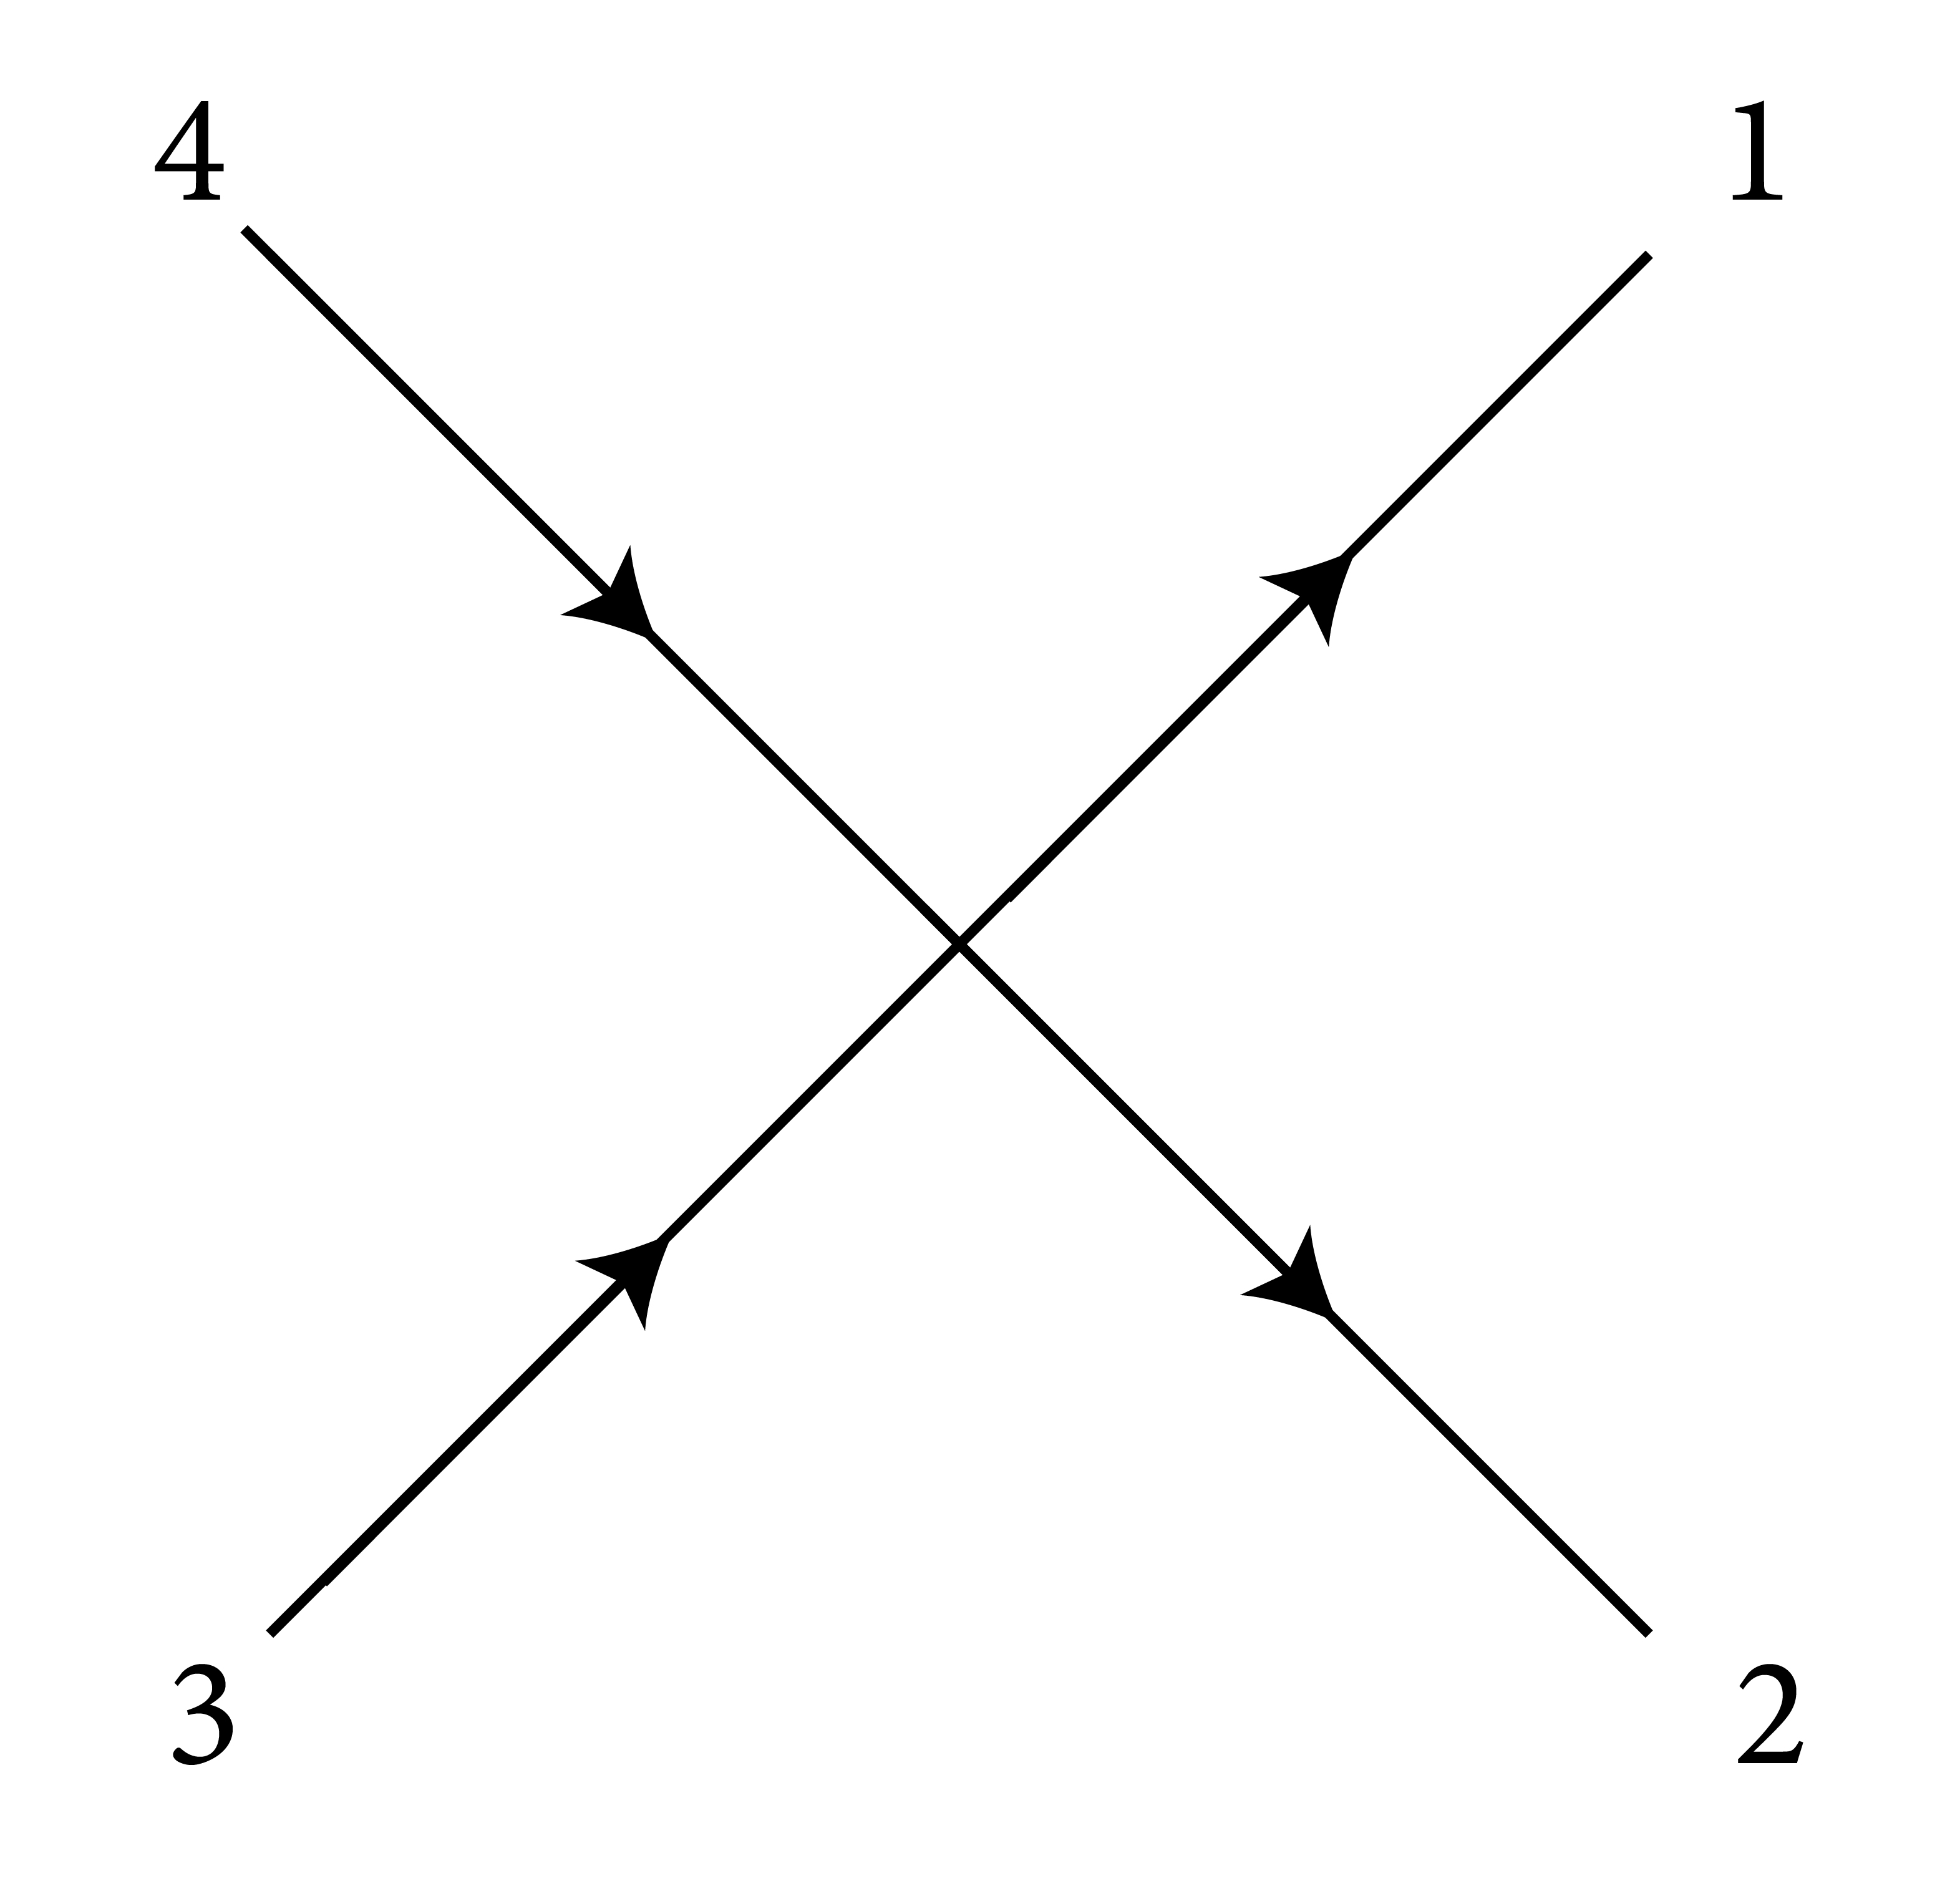
\includegraphics[width=0.4\textwidth]{images/quarticvertex.jpg}
    \caption{Lowest order diagram for the four points function.}
    \label{fig:treefourpoints}
\end{figure}
The corresponding expression is
\begin{equation}
    \langle \aonet \atwot \athreestart\afourstart \rangle_{0} = -4\frac{i}{2} \Tint_{1234}\left(\dfrac{1}{\G_1^*\F_1^{}}+\dfrac{1}{\G_2^*\F_2^{}}-\dfrac{1}{\G_3^{}\F_3^{}}
    -\dfrac{1}{\G_4^{}\F_4^{}}\right)\D_1^0\D_2^0\D_3^0\D_4^0 2\pi \delta(\delomegatt^{12}_{34})\delta^{12}_{34},
    \label{4pointfreq}
\end{equation}
where $\tilde{a}_i^{}$ is the Fourier transform of $a_i^{}(t_i)$ and the factor of four comes again from the different ways of attaching "incoming" and "outcoming" 
propagators to the vertex.\\
As we are interested in the time domain let us antitransform the four point function, already fixing $t_1 = t_2 = t_3 = t_4 = t$. The objective is
\begin{equation}
    \langle\aone(t) \atwo(t) \athreestar(t) \afourstar(t) \rangle_0 = \int \frac{d\omgatt_1}{2\pi}\frac{d\omgatt_2}{2\pi}\frac{d\omgatt_2}{2\pi}\frac{d\omgatt_2}{2\pi}
    e^{i(\omgatt_1 + \omgatt_2  -\omgatt_3 - \omgatt_4)t} \langle \aonet \atwot \athreestart\afourstart \rangle_{0}.
    \label{antitransform4}
\end{equation}
We substitute \eqref{4pointfreq} into it and use the delta function over frequencies to solve one of the three integrals. Then the remaning three integrals may 
be performed by properly closing the integration path and using the residue theorem. The result, again using \eqref{freenwav}, is
\begin{equation}
    \langle\aone(t) \atwo(t) \athreestar(t) \afourstar(t) \rangle_0 = 2\Tint_{1234}n_1 n_2 n_3 n_4\left( \frac{1}{n_1}+\frac{1}{n_2}-\frac{1}{n_3}-\frac{1}{n_4} \right)
    \frac{1}{\delomega^{34}_{12} + i\gamma_{1234}},
    \label{fourpointtree}
\end{equation}  
where $\gamma_{1234} = \gamma_1 + \gamma_2 + \gamma_3 + \gamma_4$. \\

There are four  one loop diagrams contributing to the four point function. Three of them, in figure \ref{fig:quarticoneloop}, are composed from two quartic vertices.
The remaining one is built from one sextic vertex.
\begin{figure}[ht]
    \centering
    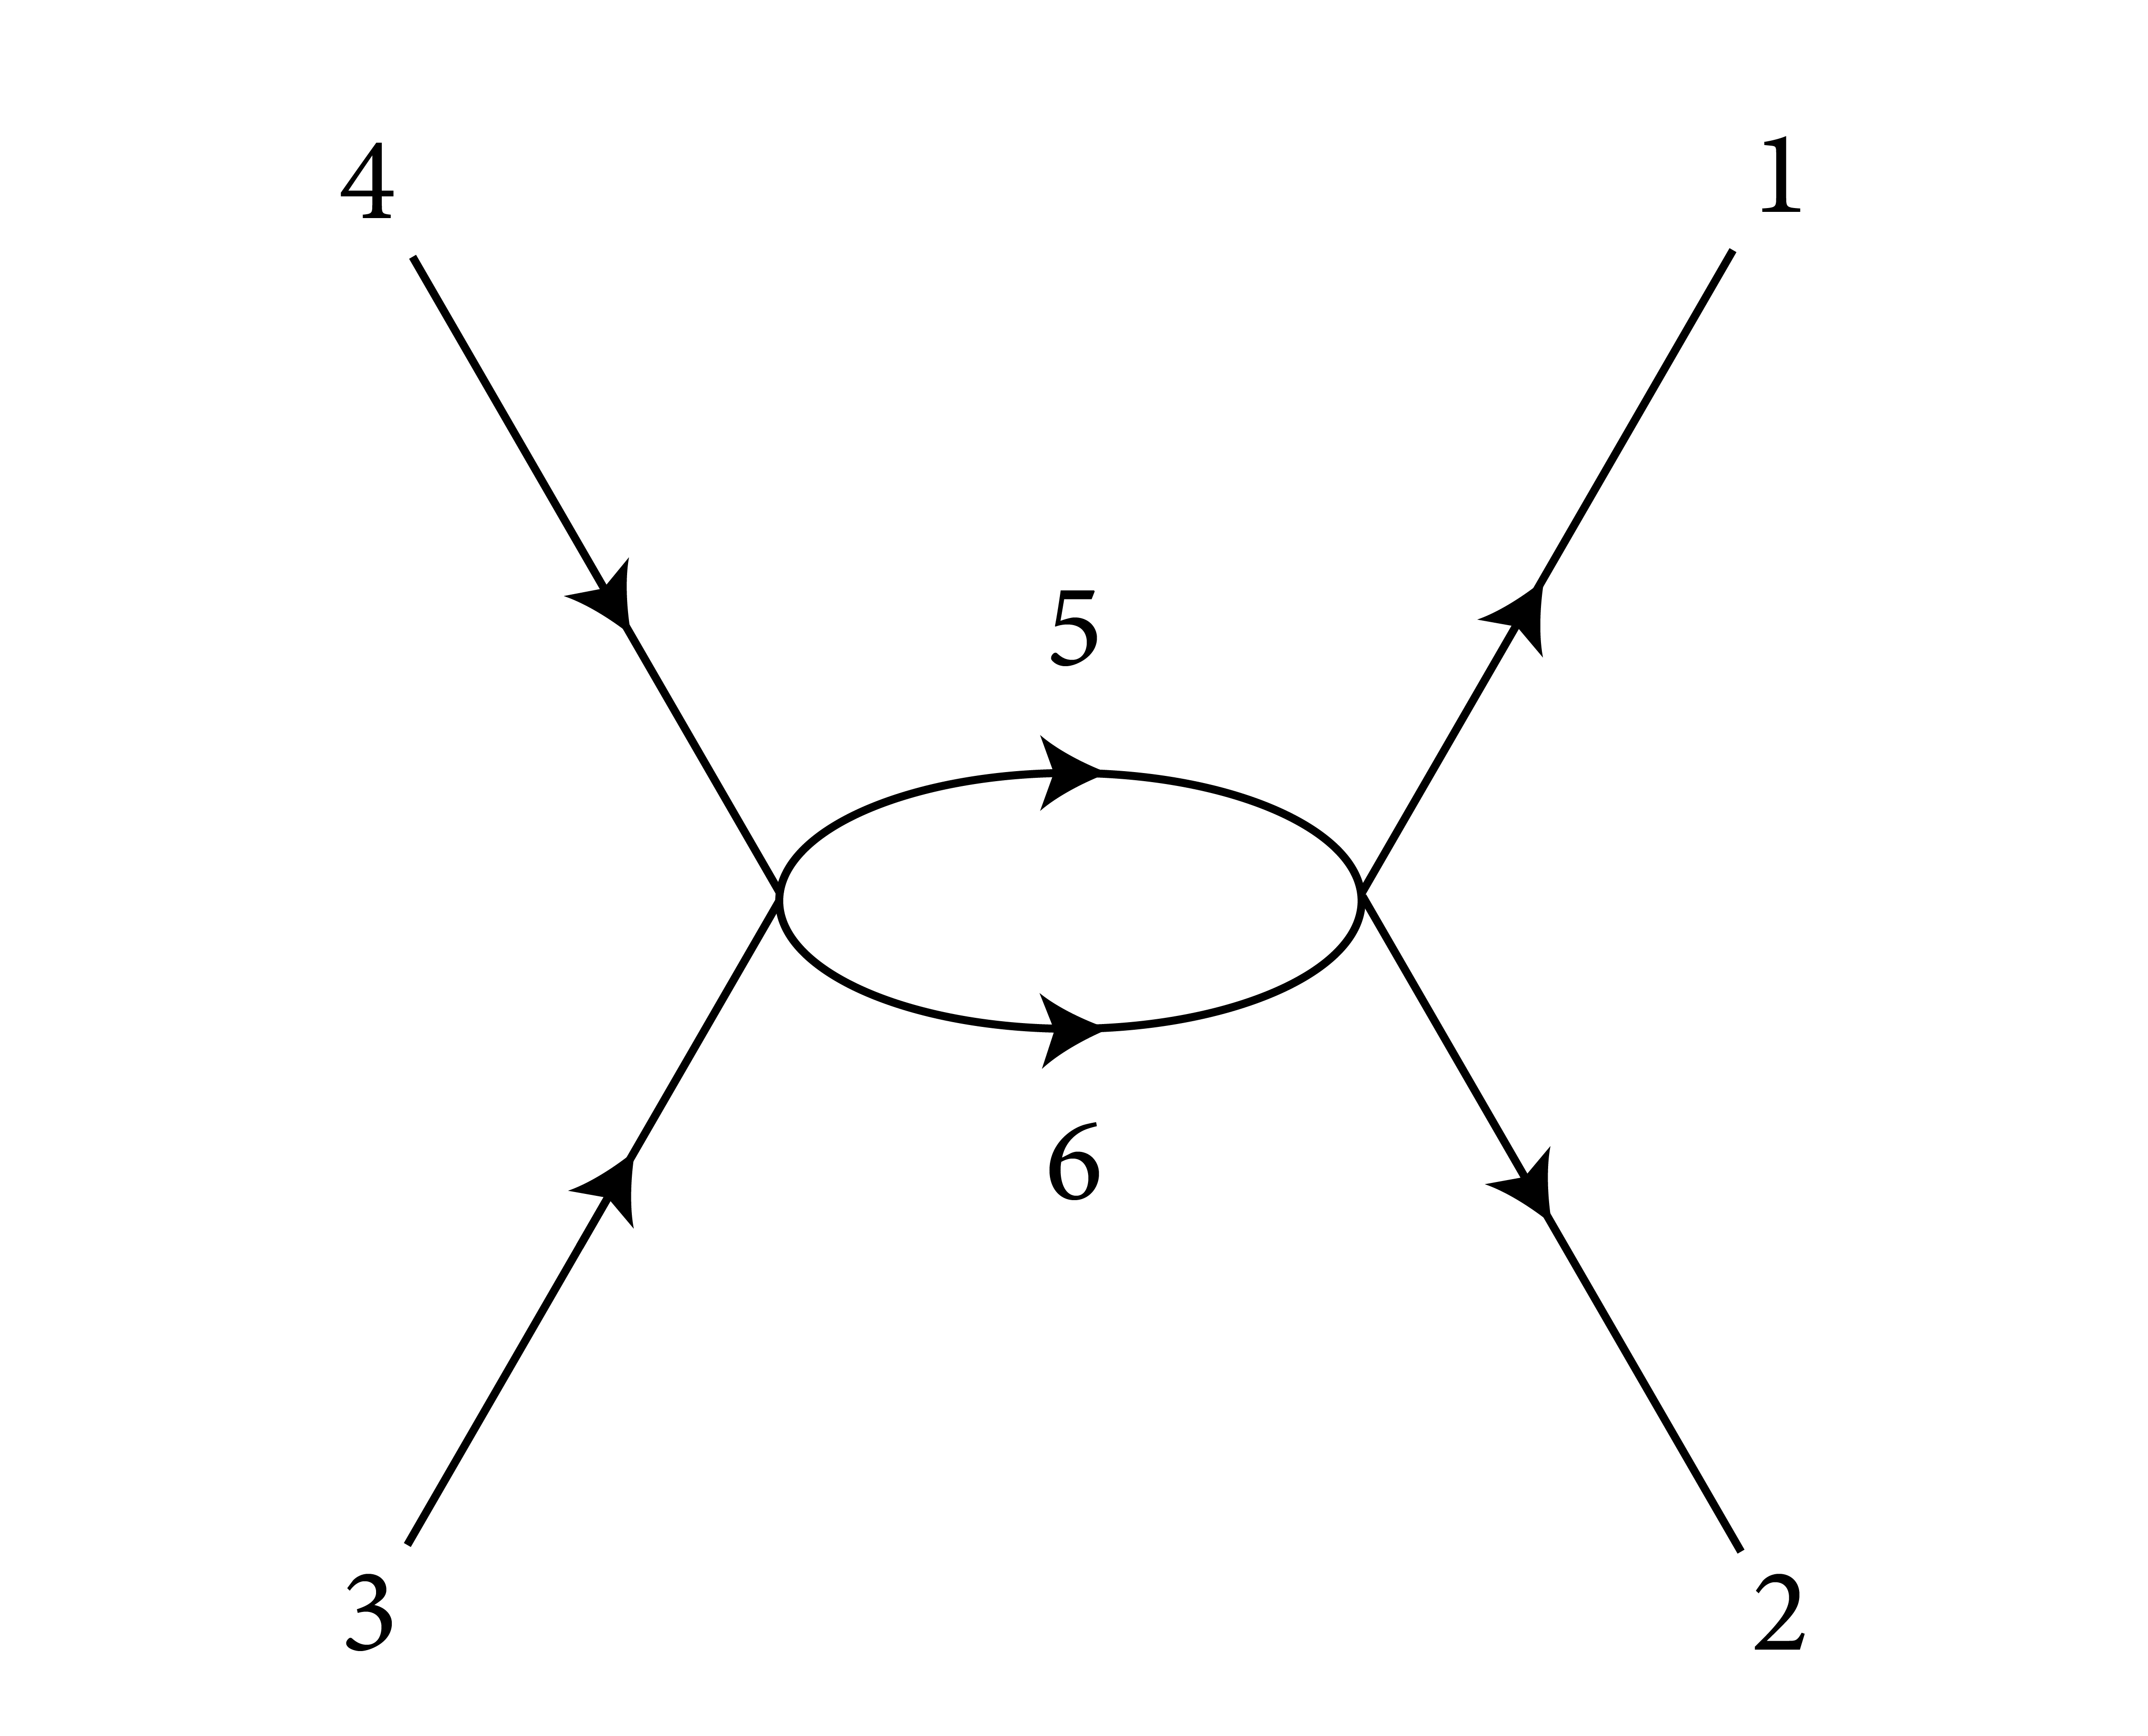
\includegraphics[width=0.4\textwidth]{images/schanneloneloop.jpg}\\
    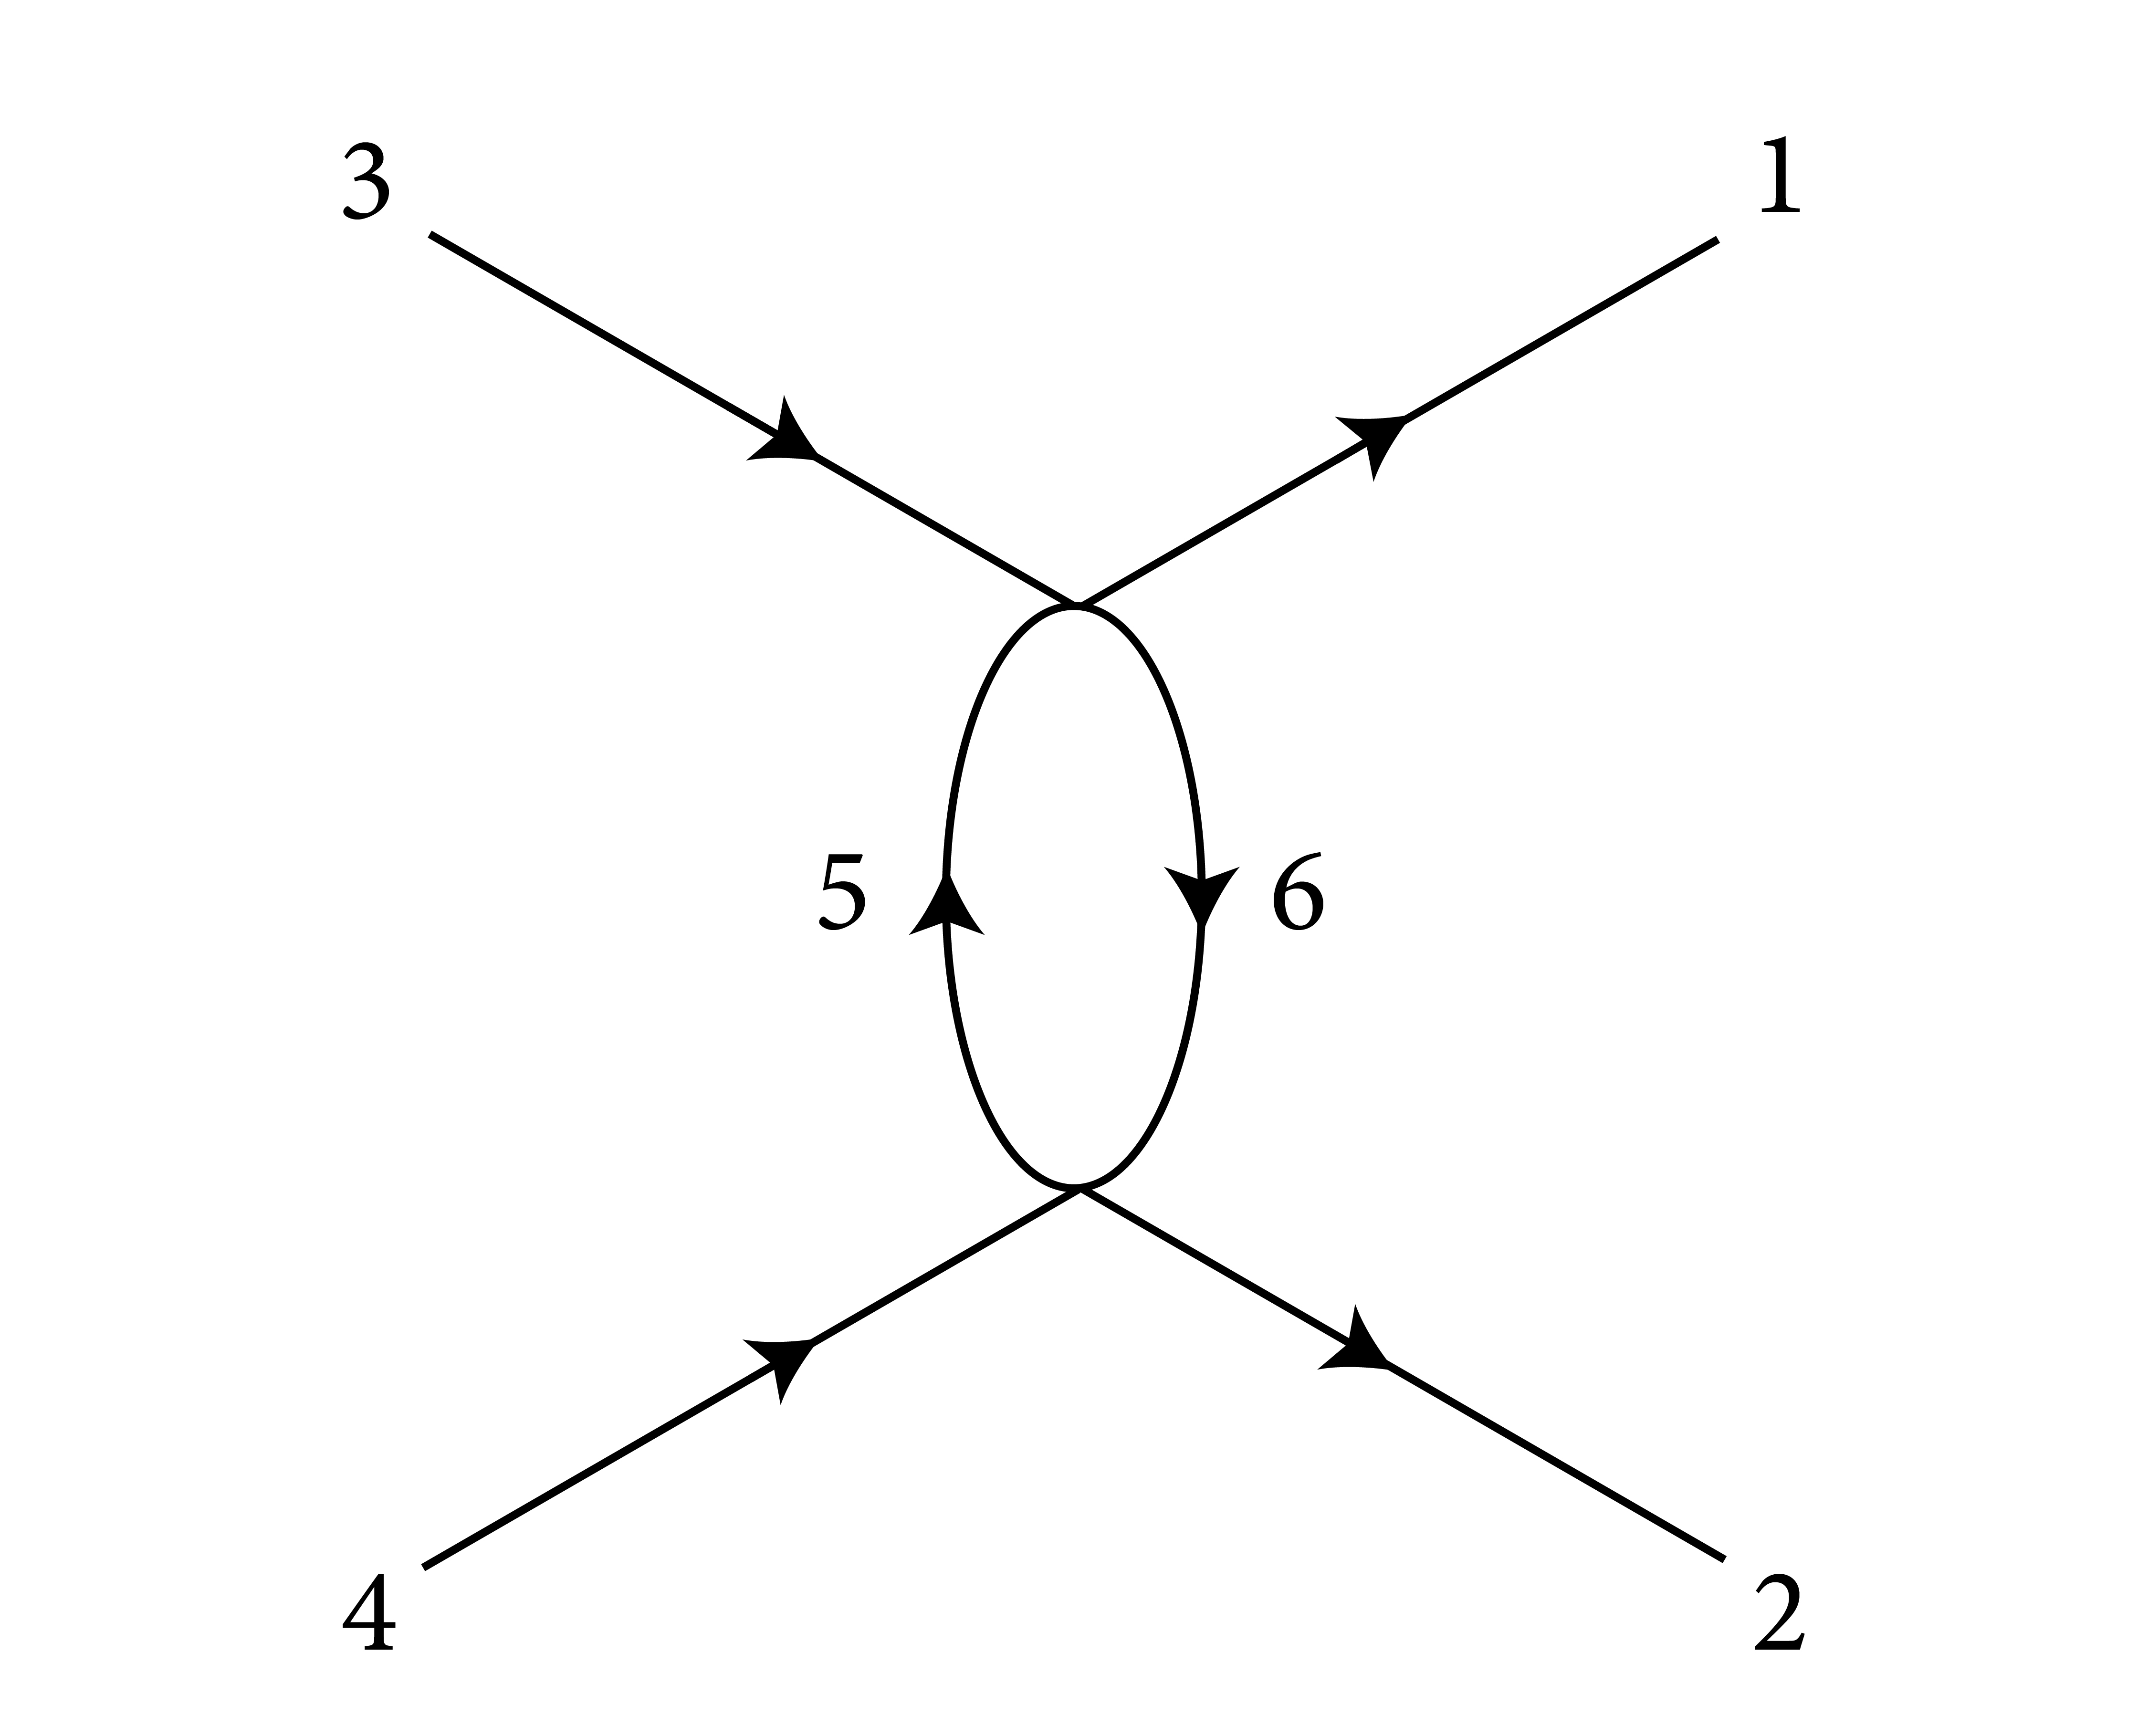
\includegraphics[width=0.4\textwidth]{images/tchanneloneloop.jpg}
    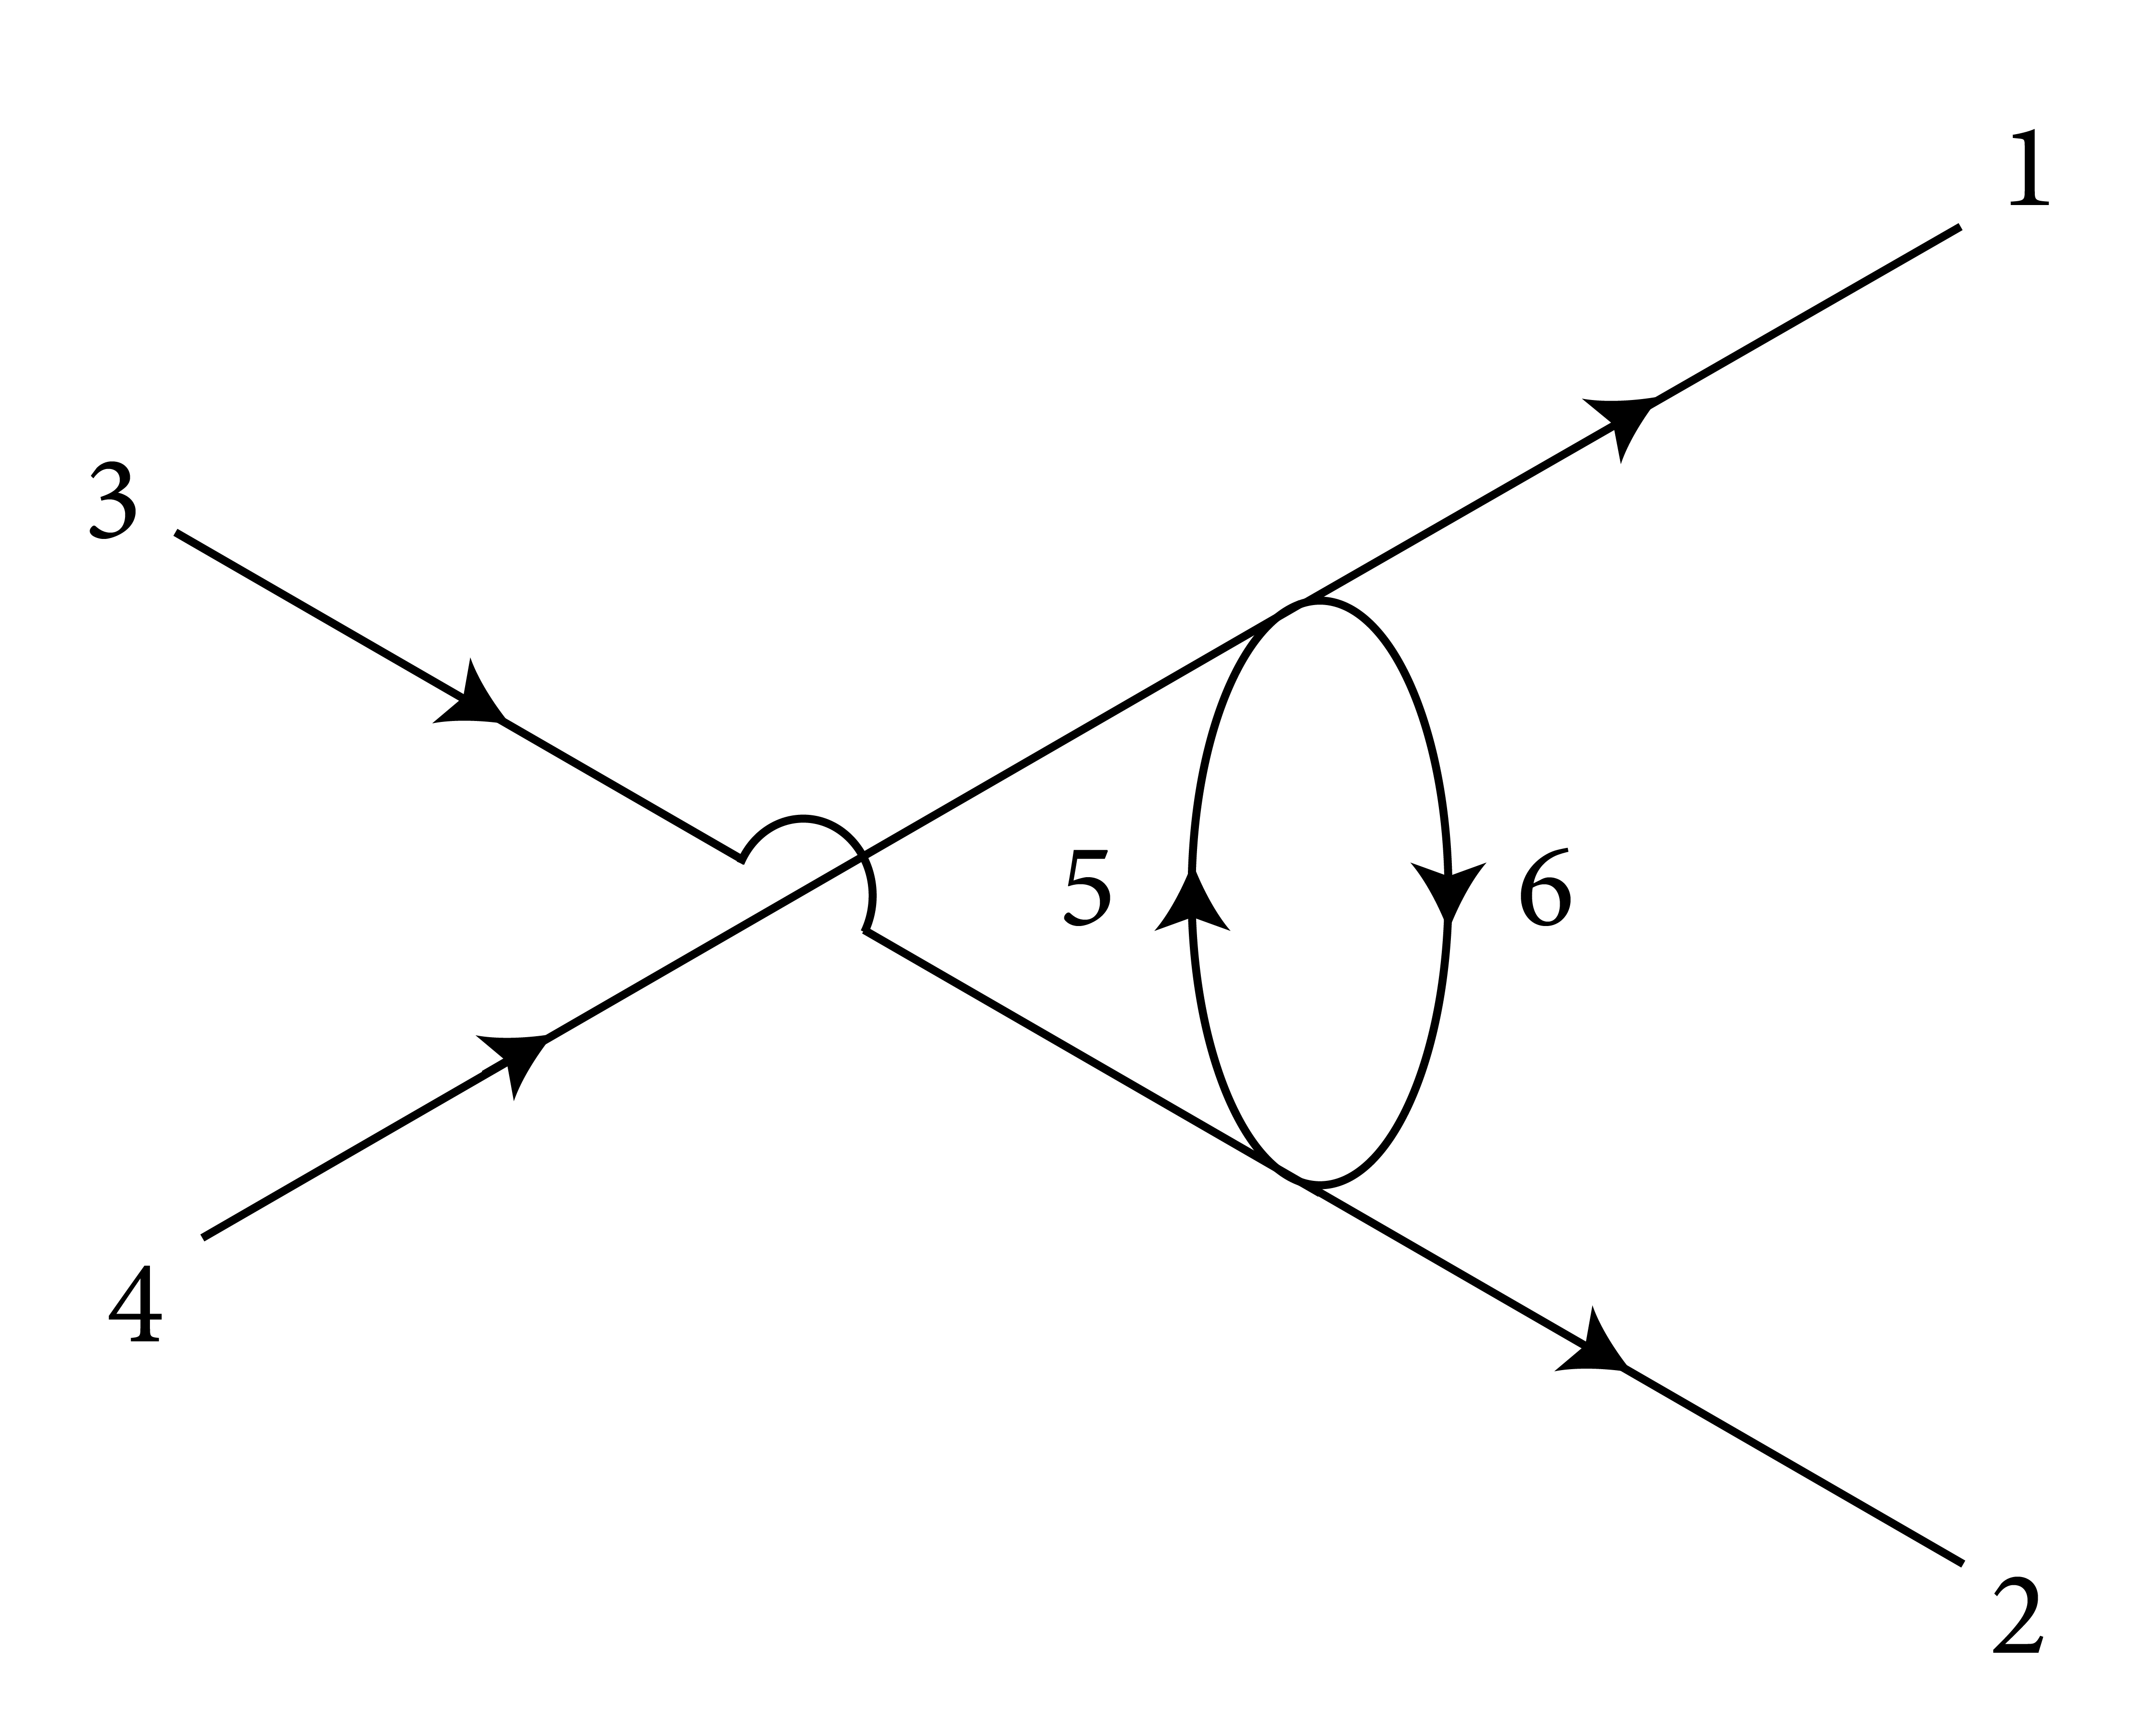
\includegraphics[width=0.4\textwidth]{images/uchanneloneloop.jpg}
    \caption{Quartic one loop diagrams.}
    \label{fig:quarticoneloop}
\end{figure} 
Let us start from the first diagram in figure \ref{fig:quarticoneloop}, it contains four external lines, two internal ones and two vertices. Its corresponding expression is
\begin{multline}
    -8\pi^2\sum_{56}\int \frac{d\omgatt_5}{2\pi}\frac{d\omgatt_6}{2\pi}\delta(\delomegatt^{34}_{56})\delta(\delomegatt^{56}_{12})\Tint_{5634}\Tint_{1256}\delta^{56}_{34}
    \delta^{12}_{56}\D_1^0\D_2^0\D_3^0\D_4^0\D_5^0\D_6^0 \\ 
    \times \left(\dfrac{1}{\G_5^*\F_5^{}}+\dfrac{1}{\G_6^*\F_6^{}}-\dfrac{1}{\G_3^{}\F_3^{}}
    -\dfrac{1}{\G_4^{}\F_4^{}}\right)\left(\dfrac{1}{\G_1^*\F_1^{}}+\dfrac{1}{\G_2^*\F_2^{}}-\dfrac{1}{\G_5^{}\F_5^{}}
    -\dfrac{1}{\G_6^{}\F_6^{}}\right).
    \label{schannel}
\end{multline}
Here the symmetry factor is given by the 16 possible ways of attaching the lines to the vertices and still results in an equivalent diagram. 
An additional factor of $\dfrac{1}{2}$ has to be included, coming from perturbation theory. The origin of this latter term is again out of the scope of this thesis, the reader is directed
to any QFT textbook to better understand it. INtuitively it corresponds to the $\dfrac{1}{2}$ term appearing in the second order of a Taylor expansion. \\
We may readily resolve one of the integrals by using a delta function, so that now $\omgatt_6 = \omgatt_3 + \omgatt_4 - \omgatt_5$. The second delta will now not depend 
anymore on the integration variable $\omgatt_5$, only enforcing conservation of energy. \\
The integrand is made of 16 terms summed, before integrating them explicitely we shall prepare some identities. We will need all possible combinations of 
the terms in \eqref{schannel} depending on $\omgatt_5$, remembering that, thanks to the delta function, $\G_6$ and $\D_6$ depends on it as well\footnote{
    Remember that $\frac{1}{\F_i \G_i}\D^{}_i = \G_i^*$, implying that $\G^{}_i$ or $\G^{*}_i$ will always appear in the numerator.
}. \\
All following identities can be easily obtained by substituting the definitions of $\D$ and $\G$, and subsequently closing the integration path either 
on the upper half plane (UHP) or the lower one (LHP). They are
\begin{align}
    &\int \frac{d\omgatt_5}{2\pi} \D_5 \D_6 \underset{LHP}{=} \frac{2n_5n_6\gamma_{56}}{\left( \omgatt_3 + \omgatt_4 - \omga_5 - \omga_6\right)^2 + \gamma^2_{56}}, 
    \label{identity1}\\
    &\int \frac{d\omgatt_5}{2\pi} \G_5 \D_6 \underset{UHP}{=} \frac{in_6}{\omgatt_3 + \omgatt_4 - \omga_5 - \omga_6 +i\gamma_{56}}, \\
    &\int \frac{d\omgatt_5}{2\pi} \G_6 \D_5 \underset{LHP}{=} \frac{in_5}{\omgatt_3 + \omgatt_4 - \omga_5 - \omga_6 +i\gamma_{56}}, \\
    &\int \frac{d\omgatt_5}{2\pi} \G_5^{} \G_6^* \underset{UHP}{=} 0, \\
    &\int \frac{d\omgatt_5}{2\pi} \D_5 \underset{LHP}{=} n_5, \label{identity5}\\
    &\int \frac{d\omgatt_5}{2\pi} \G_5\G_6 \underset{LHP}{=} \frac{-i}{\omgatt_3 + \omgatt_4 - \omga_5 - \omga_6 +i\gamma_{56}}.
    \label{identity6}
\end{align}  
Now let us move to the full integral. There is a common factor of
\begin{equation*}
    -4\pi\delta(\delomegatt^{34}_{12})\sum_{56}\Tint_{5634}\Tint_{1256}\D_1^0\D_2^0\D_3^0\D_4^0
\end{equation*}
in front of the integral. Then there is the $d\omgatt_5$ integration of 16 terms. Integrating them, using identities \eqref{identity1}-\eqref{identity6},
is a tedious but straightforward process. \hl{FORSE AGGIUNGI IN APPENDICE CONTI} The complete result is 
\begin{multline}
    -4\pi\delta(\delomegatt^{34}_{12})\sum_{56}\Tint_{5634}\Tint_{1256}\D_1^0\D_2^0\D_3^0\D_4^0 \left\{ -\frac{n_6}{\F_5}-\frac{n_5}{\F_6}\right. + 
    \frac{1}{\left( \omgatt_3 + \omgatt_4 - \omga_5 - \omga_6\right)^2 + \gamma^2_{56}}\\
    \times \left[
    i(n_5 + n_6)\left(\dfrac{1}{\G_1^*\F_1^{}}+\dfrac{1}{\G_2^*\F_2^{}}-\dfrac{1}{\G_3^{}\F_3^{}}
    -\dfrac{1}{\G_4^{}\F_4^{}}\right)\left( \omgatt_3 + \omgatt_4 - \omga_5 - \omga_6\right) + 
    \right.\\
    \left.\left.
    \gamma_{56}\left((n_5 + n_6)\left(\dfrac{1}{\G_1^*\F_1^{}}+\dfrac{1}{\G_2^*\F_2^{}}+\dfrac{1}{\G_3^{}\F_3^{}}
    +\dfrac{1}{\G_4^{}\F_4^{}}\right) - 2n_5n_6 \left(\dfrac{1}{\G_1^*\F_1^{}}+\dfrac{1}{\G_2^*\F_2^{}}\right)\left(\dfrac{1}{\G_3^{}\F_3^{}}
    +\dfrac{1}{\G_4^{}\F_4^{}}\right)\right)
    \right]\right\}.
    \label{schannelfullcontribution}
\end{multline}
The second diagram in figure \ref{fig:quarticoneloop} contains the same elements, but with permuted indexes. Its mathematical form is 
\begin{multline}
    -16\pi^2\sum_{56}\int \frac{d\omgatt_5}{2\pi}\frac{d\omgatt_6}{2\pi}\delta(\delomegatt^{46}_{52})\delta(\delomegatt^{35}_{16})\Tint_{2546}\Tint_{3516}\delta^{25}_{46}
    \delta^{35}_{16}\D_1^0\D_2^0\D_3^0\D_4^0\D_5^0\D_6^0 \\ 
    \times \left(\dfrac{1}{\G_5^*\F_5^{}}+\dfrac{1}{\G_2^*\F_2^{}}-\dfrac{1}{\G_6^{}\F_6^{}}
    -\dfrac{1}{\G_4^{}\F_4^{}}\right)\left(\dfrac{1}{\G_1^*\F_1^{}}+\dfrac{1}{\G_6^*\F_6^{}}-\dfrac{1}{\G_5^{}\F_5^{}}
    -\dfrac{1}{\G_3^{}\F_3^{}}\right).
    \label{tchannel}
\end{multline}
The ways to compose the diagram are 32, resulting in a symmetry factor of 16. Integrating through 
identities similar to \eqref{identity1}-\eqref{identity6}, the expression becomes
\begin{multline}
    -8\pi\delta(\delomegatt^{34}_{12})\sum_{56}\Tint_{2546}\Tint_{6135}\D_1^0\D_2^0\D_3^0\D_4^0 \left\{ -\frac{n_6}{\F_5}-\frac{n_5}{\F_6}\right. +
    \frac{1}{\left( \omgatt_1 + \omga_6 - \omgatt_3 - \omga_5\right)^2 + \gamma^2_{56}}\\
    \times \left(
    i(n_6-n_5)\left(\dfrac{1}{\G_1^*\F_1^{}}+\dfrac{1}{\G_2^*\F_2^{}}-\dfrac{1}{\G_3^{}\F_3^{}}
    -\dfrac{1}{\G_4^{}\F_4^{}}\right)\left(\omgatt_1 + \omga_6 - \omgatt_3 - \omga_5\right) + 
    \right.\\
    \left.\left.
    \gamma_{56}\left[(n_6-n_5 )\left(\dfrac{1}{\G_1^*\F_1^{}}-\dfrac{1}{\G_2^*\F_2^{}}-\dfrac{1}{\G_3^{}\F_3^{}}
    +\dfrac{1}{\G_4^{}\F_4^{}}\right) + 2n_5n_6 \left(\dfrac{1}{\G_2^*\F_2^{}}-\dfrac{1}{\G_4^{}\F_4^{}}\right)\left(\dfrac{1}{\G_1^*\F_1^{}}-\dfrac{1}{\G_3^{}\F_3^{}}
    \right)\right)
    \right]\right\}.
    \label{tchannelfullcontribution}
\end{multline}    
The third diagram is equal to the second one, just with the two outgoing lines swapped. Consequently its contribution can be obtained from 
\eqref{tchannelfullcontribution} by the permutations $k_3 \leftrightarrow k_4$, $\omgatt_3 \leftrightarrow\omgatt_4$ and $\omga_3 \leftrightarrow\omga_4$.\\

The last contribution to be considered at order $\Tint^2$ is the one in figure \ref{fig:sexticoneloop}. It may be regarded at the equivalent of the diagram in figure 
\ref{fig:oneloop2}, but for four points functions. We may already suspect it to be related to frequency renormalization.\\

\begin{figure}[ht]
    \centering
    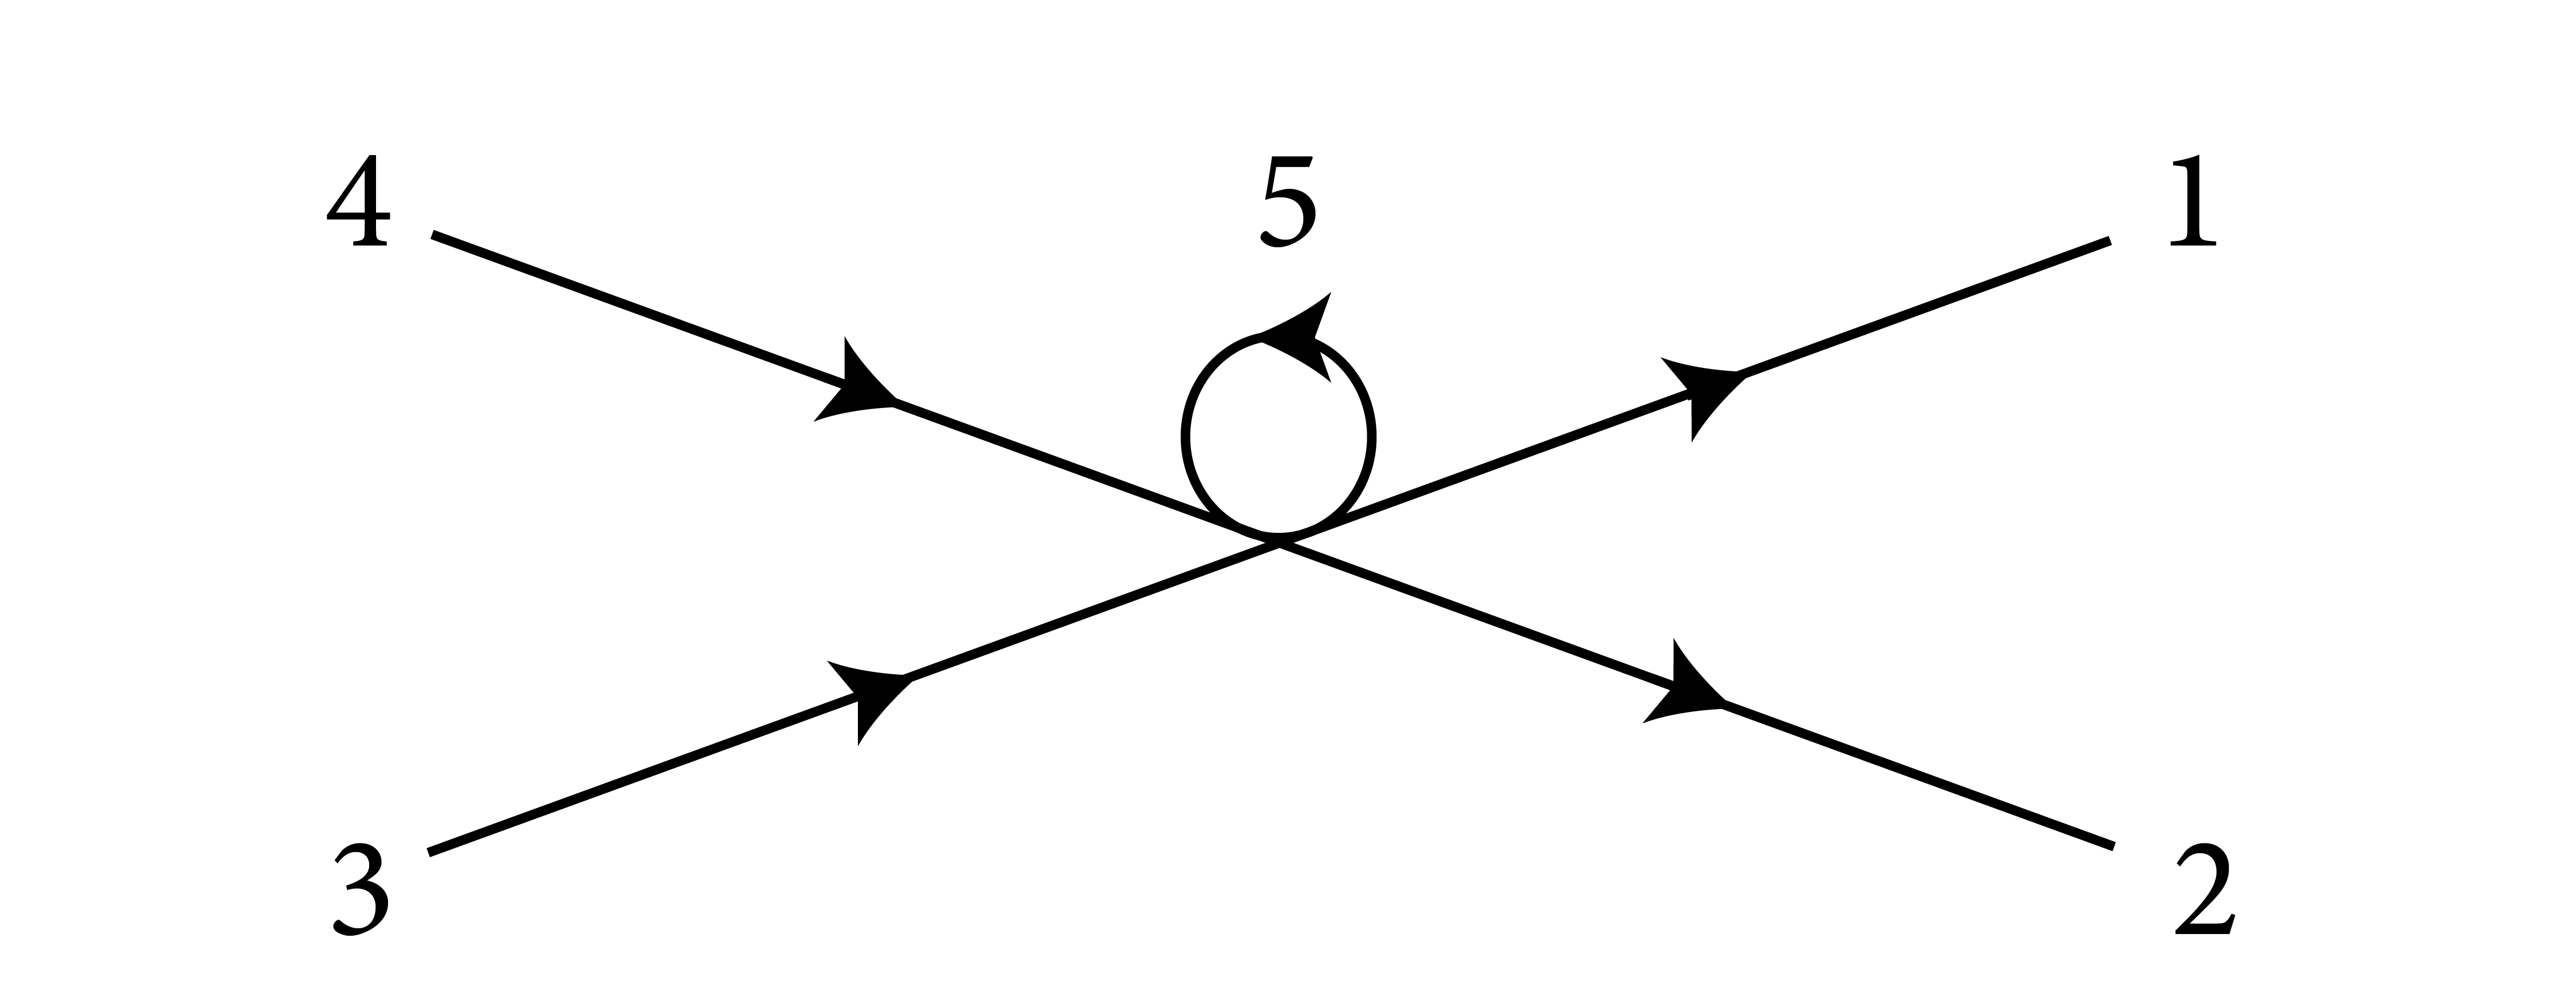
\includegraphics[width=0.5\textwidth]{images/sexticdiagram.jpg}
    \caption{Sextic one loop diagram.}
    \label{fig:sexticoneloop}
\end{figure}
We have again to consider all possible ways of attaching lines to vertices, there are \\$3!\cdot3! = 36$. However in this case different ways of building the diagram do not correspond to 
equal mathematical expressions. In the case of the first diagram in figure \ref{fig:quarticoneloop} the exchange of incoming lines would result in a term $\Tint_{2156}$
instead of $\Tint_{1256}$. Thanks to the symmetry properites of $\Tint$ the two contributions are equal and all possible permutations are accounted for in the symmetry factor.
This generalizes to quartic diagrams as the permutations always involve indexes under whose exchange the coupling $\Tint$ is symmetryc.\\ 
In the case of figure \ref{fig:sexticoneloop} it is not true that all permutations result in the same contribution, we have thus to parse through them all. The diagram 
is made of four external lines, one internal one and a sextic vertex. We exchange labels $4$ and $5$ in the sextic vertex feynman rules, as to have lines $3$ and 
$4$ both incoming as in figure \ref{fig:sexticoneloop}. The relative expression is thus  
\begin{equation}
    -2\pi \sum_{k5}\int\frac{d\omgatt_5}{2\pi} \frac{1}{\F_k}\left(\Tint_{123k}\Tint_{k545}\delta^{12}_{3k}
    \delta^{k5}_{45} + \text{permutations}\right)\delta(\delomegatt^{12}_{34})
    \D_1^0\D_2^0\D_3^0\D_4^0\D_5^0.
\end{equation}
We can resolve the integral over $\omgatt_5$, as the only term depending on it is $\D_5$, using identity \eqref{identity5}. The result is
\begin{equation}
    -2\pi \delta(\delomegatt^{12}_{34})\D_1^0\D_2^0\D_3^0\D_4^0 \sum_{k5}
    \frac{n_5}{\F_k}\left(\Tint_{123k}\Tint_{k545}\delta^{12}_{3k}
    \delta^{k5}_{45} + \text{permutations}\right).
\end{equation}
Writing all possible permutations of indexes $(1,2,5)$ and $(3,4,6)$ from $\Tint_{123k}\Tint_{k546}$, imposing $k_5 = k_6$ and using the symmetries of $\Tint$ 
reduces the unequivalent terms' number to seven. In four of them one of the deltas over wavenumbers may be used to eliminate the integration over $k$. After slightly manipulating
and renaming the dummy indexes, the full result is 
\begin{multline}
    -2\pi \delta(\delomegatt^{12}_{34})\D_1^0\D_2^0\D_3^0\D_4^0\left[ 4\sum_5\Tint_{1234}\delta^{12}_{34} \sum_{j=1}^{4}\frac{\Tint_{j5j5}}{\F_j}n_5 + \right.\\ 
    \left.  2\sum_{56}\left( \frac{n_5}{\F_6} + \frac{n_6}{\F_5} \right)\left( \Tint_{1256}\Tint_{5634}\delta^{12}_{56}\delta^{56}_{34} 
    + 2\Tint_{2546}\Tint_{6153}\delta^{25}_{46}\delta^{61}_{53}
    + 2\Tint_{5146}\Tint_{6253}\delta^{51}_{46}\delta^{62}_{53} \right) \right].
    \label{sexticfullcontribution}
\end{multline}
\\
We can rewrite the first part of \eqref{sexticfullcontribution}, using \eqref{shiftilritorno}, as 
\begin{equation}
    -4\pi \delta(\delomegatt^{12}_{34})\D_1^0\D_2^0\D_3^0\D_4^0\sum_{j=1}^{4}\frac{\delta \omga_i}{\F_i}.
    \label{shiftsextic}
\end{equation}
If we were to peform the frequency shift in $\Lag$, a new quartic interaction term would appear along with its Feynman's rule. 
This term would manifest itself, at this order of perturbation theory, in a diagram similar to the one in figure \ref{fig:treefourpoints}, 
yealding exactly the same contribution as \eqref{shiftsextic}. As we did for the diagram in figure \ref{fig:oneloop2}, we can ignore this contribution by including
the frequency shift into the final result. \\
We notice that the second part of \eqref{sexticfullcontribution} diverges in the $\F_k \rightarrow 0$ limit. Looking at the diverging contributions of 
\eqref{schannelfullcontribution}, \eqref{tchannelfullcontribution} and \eqref{tchannelfullcontribution}($3 \leftrightarrow 4$), we see that their sum is\\
\hl{FROM HER ON ADD DELTAS NEXT TO INTERACTION TERMS}
\begin{equation}
    4\pi\delta(\delomegatt^{12}_{34})\D_1^0\D_2^0\D_3^0\D_4^0\sum_{56}\left( \frac{n_5}{\F_6} + \frac{n_6}{\F_5}\right)\left(
    \Tint_{5634}\Tint_{1256} + 2 \Tint_{2546}\Tint_{6135} + 2\Tint_{2536}\Tint_{6145}
    \right).
\end{equation}
Since $k_5$ and $k_6$ are integrated over, it is easy to show that this term exactly cancels the diverging part of \eqref{sexticfullcontribution}.\\
Finally the full contribution to order $\Tint^2$ is obtained by summing the finite parts of the expressions calculated from figure \ref{fig:quarticoneloop}.
To recover the original nonlinear theory we remove the forcing and dissipating terms by taking the limit $F_k, \gamma_k \rightarrow 0$ while keeping their ratio constant
(as to have $n_k$ finite). We shall keep the $\gamma_k$ terms in the denominator as $\varepsilon$ quantities to aid with the future Fourier antitransform. The result is 
\begin{equation}
    \begin{aligned}
    \langle\aonet &\atwot\athreestart\afourstart \rangle_1 = 
    \\
    %-&2\pi i \delta(\delomegatt^{12}_{34})\Tint_{1234}\D^0_1\D^0_2\D^0_3\D^0_4\left(
    %\dfrac{1}{\G_1^*\F_1^{}}+\dfrac{1}{\G_2^*\F_2^{}}-\dfrac{1}{\G_3^{}\F_3^{}}-\dfrac{1}{\G_4^{}\F_4^{}}\right) 
    %\\
    -&4\pi \delta(\delomegatt^{12}_{34})\D^0_1\D^0_2\D^0_3\D^0_4 \times
    \\
      \sum_{56}&\left[\Tint_{5634}\Tint_{1256}
    \frac{i(n_5 + n_6)\left(\dfrac{1}{\G_1^*\F_1^{}}+\dfrac{1}{\G_2^*\F_2^{}}-\dfrac{1}{\G_3^{}\F_3^{}}
    -\dfrac{1}{\G_4^{}\F_4^{}}\right)\left( \omgatt_3 + \omgatt_4 - \omga_5 - \omga_6\right)}{\left( \omgatt_3 + \omgatt_4 - \omga_5 - \omga_6\right)^2 + \gamma^2_{56}}
    +  \right.
    \\
    &\hspace{2mm}\left. \Tint_{2546}\Tint_{6135}
    \frac{i(n_6 - n_5)\left(\dfrac{1}{\G_1^*\F_1^{}}+\dfrac{1}{\G_2^*\F_2^{}}-\dfrac{1}{\G_3^{}\F_3^{}}
    -\dfrac{1}{\G_4^{}\F_4^{}}\right)\left( \omgatt_3 + \omgatt_4 - \omga_5 - \omga_6\right)}{\left( \omgatt_1 + \omga_6 - \omgatt_3 - \omga_5\right)^2 + \gamma^2_{56}}
    + \left( 3 \longleftrightarrow 4 \right) \right].
    \end{aligned}
    \label{transformedfourpoint}
\end{equation}
To Fourier transform this expression is a rather straightforward but cumbersome task. In doing so it is useful to have kept the $gamma$ in the denominator. 
By sending them to zero uniformely in $k$-space one can substitute $\gamma_k= \frac{\varepsilon}{4}$ and avoid singularities on the integration path. It is however important 
to check that the integral is converging without the $\varepsilon$ term. Transforming in the same fashion as \eqref{antitransform4}, we obtain 
\begin{multline}
    \langle \ak(t) \aone(t) \atwostar(t)\athreestar(t) \rangle_{1} = 2\sum_{56} \left( \Tint_{5634}\Tint_{1256}  V(1,2,3,4,5,6) - \right.\\
    2\Tint_{2546}\Tint_{6135}
    \left.V(1,-3,-2,4,5,-6) - 2\Tint_{2536}\Tint_{6145} V(1,-4,-2,3,5,-6)  \right),
\end{multline}
where 
\begin{equation}
    \begin{aligned}
        V(1,2,3,4,5,6) =&
        \\
        -\prod_{j=1}^{6}n_j\left[ \vphantom{\frac{1}{n_7}} \right.
        &\left( \frac{1}{n_1} +\frac{1}{n_2} \right) \left( \frac{1}{n_3} +\frac{1}{n_4} \right)
        \left( \frac{1}{\delomega^{34}_{56} + i\varepsilon}\frac{1}{\delomega^{56}_{12} + i\varepsilon} - \pi^2\delta(\delomega^{34}_{56})\delta(\delomega^{56}_{12})\right)-  
        \\
        &\left( \frac{1}{n_1} +\frac{1}{n_2} \right) \left( \frac{1}{n_5} +\frac{1}{n_6} \right)
        \frac{1}{\delomega^{34}_{12} + i\varepsilon}\frac{1}{\delomega^{34}_{56} + i\varepsilon} -
        \\
        &\left( \frac{1}{n_3} +\frac{1}{n_4} \right) \left( \frac{1}{n_5} +\frac{1}{n_6} \right)
        \frac{1}{\delomega^{34}_{12} + i\varepsilon}\left.\frac{1}{\delomega^{56}_{12} + i\varepsilon}
        \right]
    \end{aligned}
\end{equation}

\subsection{Higher order kinetic equation}

Having calculated the four point function up to $\Tint^2$ order, we may use it in conjunction with \eqref{kineticprototype} to derive an higher order kinetic equation.\\
It is straightforward to see that substituting \eqref{fourpointtree} into \eqref{kineticprototype}, and using the known identity
\begin{equation}
    \frac{1}{f(x) + i\varepsilon} = \frac{1}{f(x)} -i\pi\delta(x),
    \label{deltaidentity}
\end{equation}
the usual kinetic equation \eqref{kinetic} is recovered. \\
In \eqref{deltaidentity} the integral of $\frac{1}{f(x)}$ has to be intended in the principal value sense, but must nontheless be converging. For example it is possible to say that the principal value 
of 
\begin{equation}
    \int_{-\infty}^{\infty}\frac{dx}{x}
\end{equation} 
is null. However it is not possible to assign finite value to 
\begin{equation}
    \int_{-\infty}^{\infty} \frac{dx}{x^2}.
\end{equation}
We stress this fact as it will be of importance in the next chapter. \\
Substituting instead \eqref{transformedfourpoint} into \eqref{kineticprototype}, after some lenghty manipulations described in the appendix of \cite{Rosenhaus2023},
we obtain Rosenhaus and Smolkin's kinetic equation (we also recover explicit integrations $\sum_5 \rightarrow \int dk_5$)
\begin{multline}
        \pt \langle \ak(t) \akstar(t) \rangle = \pt n_k(t) = 4\pi \int \prod_{j=1}^{3} dk_j|\Tint_{k123}|^2n_kn_1n_2n_3\left(\frac{1}{n_k} +\frac{1}{n_1}-
        \frac{1}{n_2}-\frac{1}{n_3}\right)\delta(\delomega^{k1}_{23}) \\
          + 16\pi\int \prod_{j=1}^{5} dk_j\delta(\delomega^{k1}_{23})n_kn_1n_2n_3n_4n_5 \\
          \times \left\{  \dfrac{\text{Re}(\Tint_{23k1}\Tint_{k145}\Tint_{4523})}{\delomega^{23}_{45}}
          \left(\frac{1}{n_k} +\frac{1}{n_1} -\frac{1}{n_2} - \frac{1}{n_3}\right)\left(\frac{1}{n_4}+\frac{1}{n_5}\right)  \right. \\
          + \frac{3}{2}\pi\text{Im}(\Tint_{23k1}\Tint_{k145}\Tint_{4523})\delta(\delomega^{23}_{45})\left(\frac{1}{n_k}+\frac{1}{n_1}\right)\left(\frac{1}{n_2}
          +\frac{1}{n_3}\right) \\
            + 4\left[\dfrac{\text{Re}(\Tint_{23k1}\Tint_{k524}\Tint_{1435})}{\delomega^{35}_{14}}
            \left(\frac{1}{n_k} +\frac{1}{n_1} -\frac{1}{n_2} - \frac{1}{n_3}\right)\left(\frac{1}{n_4}-\frac{1}{n_5}\right)\right. \\
            + \left. \left. \frac{3}{2}\pi\text{Im}(\Tint_{23k1}\Tint_{k524}\Tint_{1435})\delta(\delomega^{35}_{14})\left(\frac{1}{n_k}-
            \frac{1}{n_2}\right)\left(\frac{1}{n_1}-\frac{1}{n_3}\right)  \right]\right\}.
            \label{NLOkinetic}
\end{multline}
Up until here $n_k = \frac{\F_k}{2\gamma_k}$ was only the name given to a finite ratio, but as we saw from equation \eqref{freenwav} it is also the value of the 
wave density at first order in perturbation theory. We may consequently close the equation we just obtained by the substitution $n_i \rightarrow n_i(t) = n_i$. 
As in the first chapter, this assumption holds provided that the interaction term is truly perturbative. If this is the case, it is reasonable (but not trivial) 
to expect the theory to stay close enough to a free one as to make \eqref{NLOkinetic} valid at any time. \\ 
Into this new kinetic equation every frequency should be assumed to be shifted by the quantity $\delta\omega$, to account for the contributions of 
figure \ref{fig:oneloop2} and \ref{fig:sexticoneloop}.\\

It is easy to see that solution \eqref{Gibbs} remains an equilibrium state even for \eqref{NLOkinetic}. The same cannot be said for 
KZ states. Rosenhaus and Falkovich studied the convergence of \eqref{NLOkinetic} when one of the KZ solutions of \eqref{kinetic} is substituted into it, 
as it could be expected that if a stationary solution exist it should be close to \eqref{KZPsol} or \eqref{KZQsol}. Under some very general assumptions on the 
scaling properties of the dispersion relation and the interaction term, they found that a locality window is not to be usually expected. This implies that even if 
a solution is found for a given theory, some integral in the equation will diverge either in the infrared (IR) region or in the ultraviolet (UV) one. The only way to
heal such divergencies, that they argue become worse at higher perturbative order, is to impose IR and UV cutoffs based on the underlying physics of the problem
under consideration. This would imply that the pumping an dissipating scales influence the form of eventual cascade solutions. \\
They even managed to resum part of the most divergent diagrams, obtaining a UV convergent, but still IR divergent, kinetic equation. It is however an open question 
how much insight can be extracted about the strong turbulence regime, as it is often the case that nonperturbative effects in strongly nonlinear theories are hidden
from the point of view of perturbation theory. It is also an incognita wether the closure needed to obtain the WKE is self consistent in the case of non negligible contributions 
from the nonlinear part of the Hamiltonian. \\


%chapter3
% !TEX root = ../../thesis.tex


\newpage
\vphantom{}
\section{A one dimensional model for Wave Turbulence}

\begin{itemize}
    \item mini intro su storia MMT e outline capitolo
    \item MMT model con beta generico e sua WKE
    \item soluzioni KZ con beta generico e controllo sommario convergenza (solo limiti)
    \item trasformata di Zakharov (se già introdotta in chap 1 solo usarla) e controllo convergenza LO integrando
    \item commmenti su validita WKE data la presenza di solitoni e quasisolitoni (devi studiarla prima bro)
    \item MMT nlo, qunatità ancora conservate e discussioni sulla sua convergenza e sulla natura delle correzioni
    \item tutto quello che riusciamo a trovare come previsione teorica 
\end{itemize}




%chapter4
%% !TEX root = ../../thesis.tex


\newpage
\vphantom{}
\section{Numerical study of the Wave Kinetic Equation}

\begin{itemize}
    \item intro e obbiettivi
    \item WavKinS struttura base e funzionamento (che algoritmi usa)
    \item simulazioni leading order e commenti sulle stesse
    \item simulazioni nlo e commenti, confronti con aspettative teoriche
\end{itemize}







%%%%%%%%%%%%%%%%%%%BIBLIOGRAPHY%%%%%%%%%%%%%%%%%%%%%%%%
\newpage
%without biblatex package:
\bibliographystyle{plain}  
\bibliography{bibliog}
%%%%%%%%%%%%%%%%%%%%%%%%%%%%%%%%%%%%%%%%%%%%%%%%%%%%%%%


%%%%%%%%%%%%%%APPENDIX%%%%%%%%%%%%%%%%%%%

\end{document}






